\newif\ifprintfig
\printfigtrue
%\printfigfalse

%%---------------------------------------------------
%\documentstyle[11pt,psfig,aaspp4]{article}
%\tightenlines
%\documentclass[12pt,preprint]{aastex}
%\documentclass[manuscript]{aastex}
\documentclass{emulateapj}
\usepackage{graphicx}
\usepackage{subfigure}
%% allow png & JPG  (http://merkel.zoneo.net/Latex/index.php)
%%\usepackage{pgf}  
%%\bibliographystyle{apj}

%%---------------------------------------------------

\begin{document}

\title{PHAT:  Cluster Properties}
\author{Lori C. Beerman, Morgan Fouesneau, L. Clifton Johnson, Anil C. Seth, Julianne J. Dalcanton, Daniel R. Weisz, Ben F. Williams, Alexia R. Lewis, Yumi Choi, PHAT Collaboration} 


\begin{abstract}

We utilize the PHAT cluster sample, which is the largest uniformly derived extragalactic cluster sample to date, containing 2753 clusters.  We present results for the ages, masses, and extinctions of this cluster sample and demonstrate their accuracy through the use of synthetic clusters.  The parameter estimates were done using two  methods (CMD fitting of the resolved stars and integrated light fitting using discrete population models).  We summarize the most accurate estimates for each cluster.  These clusters span a large range of ages and masses (down to a few hundred solar masses), as well as location throughout the disk of M31.

\end{abstract}
\keywords{galaxies:  stellar content}


\vfill
\clearpage

%----------------------------------------------
%----------------------------------------------x`

\section{Introduction}\label{intro}


Stellar clusters are widely used out to $\sim$ 50 Mpc to investigate star formation, stellar evolution, and the formation histories and evolution of galaxies.  At these distances, integrated light measurements are routinely used to analyze the ages and masses of clusters.  These methods fit multi-wavelength flux measurements (usually including the UV) with predictions from models of single age stellar populations and foreground dust.  This is a mature field, with many catalogs of clusters with ages and masses derived from integrated light measurements, such as those for M83 \citep{Bastian12}, M33 \citep{SanRoman10}, the Large Magellanic Cloud \citep[LMC; ][] {Hunter03, Popescu12}, M51 \citep{Chandar11}, and the Antennae Galaxies \citep{Whitmore10}.  

Most advanced methods include discrete models, which attempt to reduce the stochastic effects that are inherent in integrated light studies.  Integrated light determinations of the cluster properties are generally fairly accurate for clusters above a few $10^4 M_{\odot}$ mass.  However, for lower mass clusters, this method suffers greatly from stochastic effects due to the clusters' luminosity being dominated by a very small number of stars, rather than by a well populated stellar mass function.  The effects of stochasticity are particularly severe at young cluster ages due to individual stars rapidly evolving off the main sequence  \citep[e.g.,][] {Lancon00, Cervino04, Apellaniz09, Piskunov09, Popescu10a, Fouesneau10, Beerman12}.  Older than a few 100 Myr, the integrated light of the cluster is dominated by more numerous lower mass stars, and thus reduces the effects of stochasticity.  While current studies that treat the mass function as a discrete distribution of stars \citep{Fouesneau12, Popescu12} do a much better job than traditional integrated light age determinations, problems remain, such as sensitivity to stellar models for rapidly evolving massive stars, and uncertain photometry due to the effects of crowding, spatially variable complex backgrounds, and dust.  

Deriving cluster properties using color-magnitude diagrams (CMDs) of resolved stars has been the gold standard.  With resolved stars, we can fit stellar models to their CMD to derive the age and extinction, and using mass-to-light ratios or stellar models, we can derive their mass as well with a greater accuracy.  These resolved studies do not suffer from the same degeneracies and stochastic effects as the integrated studies.  However, such studies can only be used in clusters that are sufficiently close that their individual stars can be resolved from one another.  

The Local Group is currently the only place where large populations of clusters can be resolved into individual stars.  It is therefore the ideal place to compare cluster property determination methods.  Such a test is possible using ground based data in the Magellanic Clouds, but these low metallicity dwarf systems are not representative of the metal-rich disk dominated systems that we observe out to further distances.  M31, however, is the perfect system for this kind of comparison study, since it is near enough that we can obtain both resolved measurements of individual stars within the clusters (using HST) and integrated light measurements of the clusters as a whole.  We can therefore compare the results from both methods and determine in what environments and for what types of clusters the methods agree and where integrated light fitting is biased or fails completely.  This comparison will ensure that surveys done at larger distances can optimize their age and mass results from integrated light fits.

The Panchromatic Hubble Andromeda Treasury  \citep[PHAT;][] {Dalcanton12} survey of M31 has the exceptional resolution and broad wavelength coverage that is required for this comparison.  The PHAT survey imaged 1/3 of M31's disk in six filters \citep{Williams14} and has been used to construct a large well-characterized sample of clusters \citep{Johnson15}.  We can resolve many individual stars within the clusters, enabling us to accurately derive their properties.  We can also identify clusters down to very low masses, guaranteeing high completeness, and a large number of clusters where the effectiveness of stochastic models can be tested.  This sample allows us to investigate both methods of determining cluster parameters and how that accuracy depends on parameter space.  Additionally, understanding the validity of the various methods will enhance the reliability of new surveys such as LEGUS \citep{Calzetti15}, which will vastly increase the samples of integrated multi-wavelength measurements of clusters in extragalactic systems.

The organization of this paper is as follows:  In Section~\ref{sec:sample} we describe the PHAT cluster sample used in this paper.  In Section~\ref{sec:properties} we describe our two methods for determining cluster properties.  Section~\ref{sec:cmd} describes the CMD fitting technique and Section~\ref{sec:intlight} describes the integrated light technique.  We present the results in Section~\ref{sec:merged}, with broad comparisons between the methods in Section~\ref{sec:broad} and common failure modes investigated in Section~\ref{sec:disagree}.  We do a by-eye check of all results in Section~\ref{sec:assign} and present a table of our final results.  We explore the age and mass distribution for our cluster sample in Section~\ref{sec:distributions} and investigate how this would change for integrated light only studies in Section~\ref{sec:intonly}.  Finally, we present our conclusions in Section~\ref{sec:conc}.




\section{Cluster Sample} \label{sec:sample}



\begin{figure}[ht!]
   \begin{center}$
      \begin{array}{cc}
         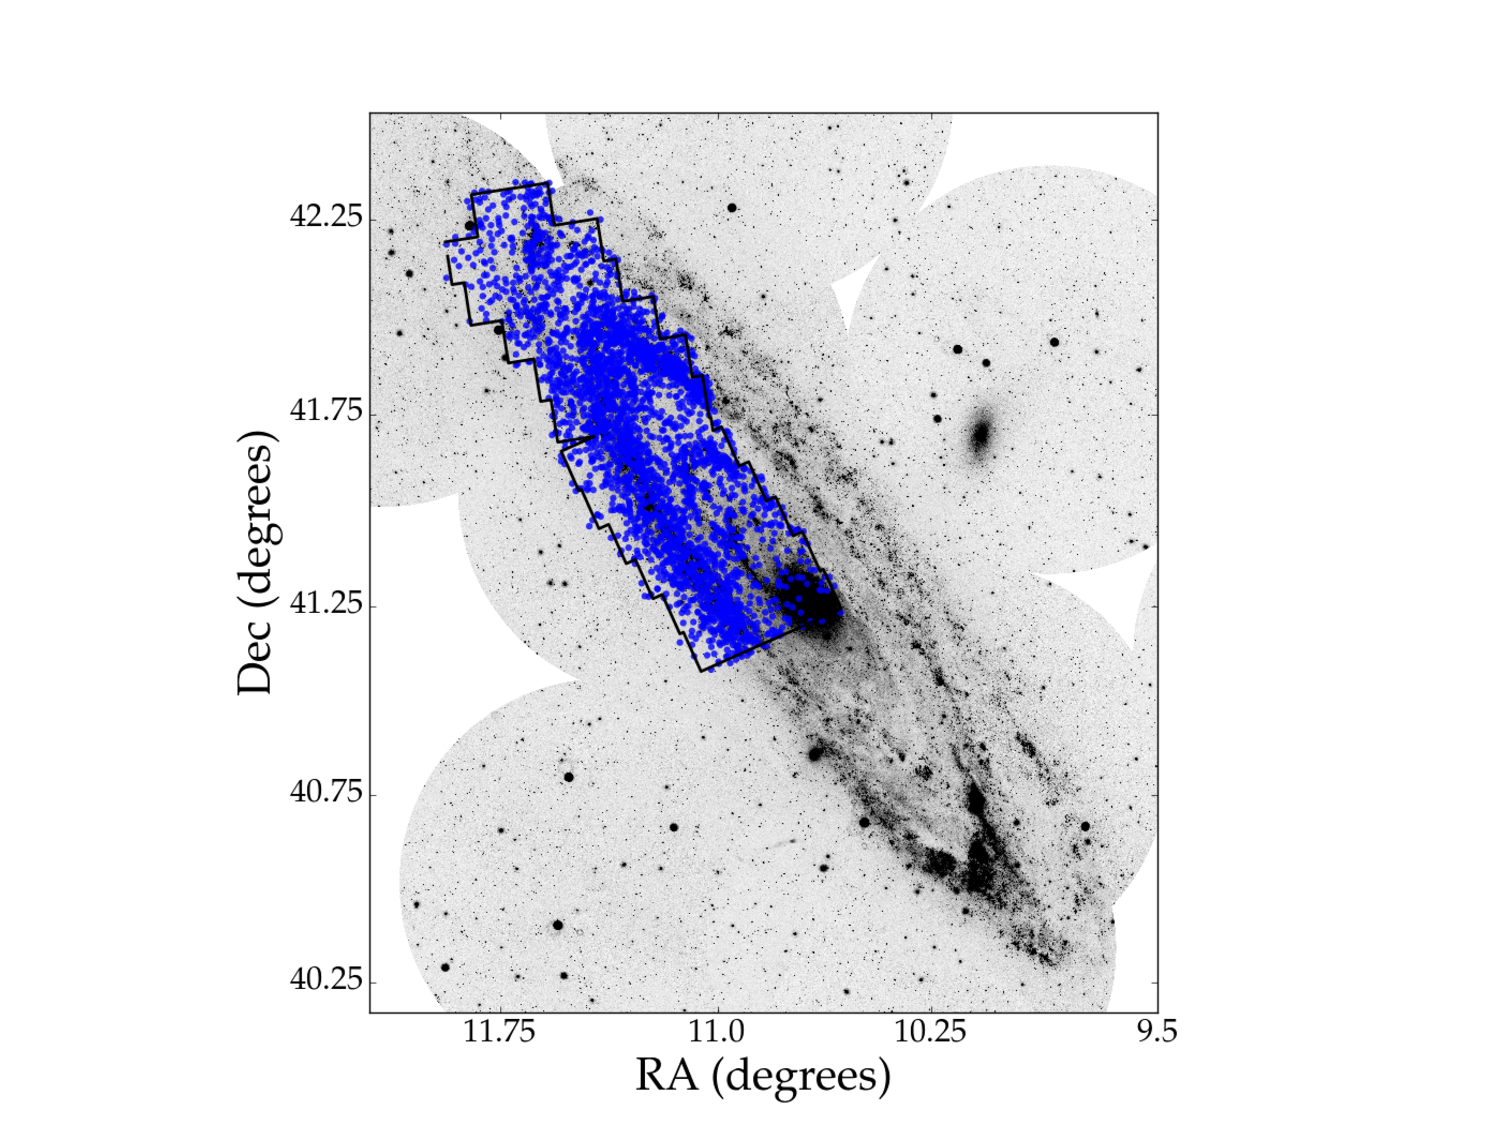
\includegraphics[trim=3.4cm 0.2cm 0.2cm 0.2cm, clip=True, scale=0.5]{cluster_catalog_footprint.pdf} 
      \end{array}$
   \end{center}
  \caption{Background GALEX NUV image of M31 \citep{Thilker05}, showing the locations of the stellar clusters (blue points) in the PHAT cluster sample. }
  \label{fig:agedist}
\end{figure}


We use the cluster sample from the PHAT survey \citep{Johnson15}. The Panchromatic Hubble Andromeda Treasury \citep[PHAT;][] {Dalcanton12} was a four year HST survey that imaged $\sim$1/3 of M31's star-forming disk and resolved over 100 million stars \citep{Williams14}.  The survey was done in six filters, covering UV to near-IR:  F275W, F336W, F475W, F814W, F110W, and F160W.  Photometry was done for individual stars brighter than $\sim$27.9 in the F475W band (for a S/N ratio of 4).  

From these images,  in collaboration with the Zooniverse citizen science team, \cite{Johnson15}, compiled a catalog of 2753 clusters using the results of a by-eye search of all the optical PHAT images.  The final cluster catalog includes many faint and sparse clusters, and increases the number of known clusters within the PHAT footprint by a factor of six.  The integrated magnitudes of clusters range over three magnitudes in the F475W band, and the luminosity function probes two orders of magnitude deeper than previous studies done in the LMC, M33, and M83.  While some of the objects in the catalog may not be bound objects, this catalog does not include larger scale (\textgreater\ 10 pc) associations of stars.  

To assess the completeness of the cluster sample, artificial clusters, with a range of ages and masses, were inserting into the images used in the by-eye search and their recovery rate was measured.  As expected, the catalog completeness is a function of both age and mass, where the sample is highly complete at M \textgreater\ $10^{3.2}M_{\odot}$ and $t$ \textgreater\ 10 Myr.  At ages \textless\ 10 Myr, many clusters may still be embedded within molecular gas, and would not have been identified by the optical image search.  Completeness is also a function of galactic environment, where clusters in the crowded inner region of M31 are more likely to be missed.  Additionally, completeness is higher for clusters \textless\ 100 Myr, since there are more stars on the main sequence, making the clusters more easily identifiable.  Artificial cluster tests show that the cluster sample is 50 percent complete down to 500 $M_{\odot}$  for clusters younger than 100 Myr.  For a complete description of the completeness of the cluster sample, see \cite{Johnson15}.


\subsection{Cluster Photometry:  Individual Stars}\label{sec:phot}

In this paper we use optical photometry for the cluster CMD fitting.  CMD fitting requires two bands, and the PHAT survey filters F475W and F814W provide the deepest photometry of the stars within each cluster.  These two filters have about 50\% more detections than in the UV or IR bands, since the UV images are about two magnitudes shallower than the optical images, and the IR suffers more from crowding due to the lower angular resolution of the WFC3/IR camera.  

The depth of the photometry depends on galactic environment and crowding, which varies from cluster to cluster.  The 50\% completeness limit varies from 26.4 to 27.8 mag in the F475W filter, and from 25.0 to 26.9 mag in the F814W filter \citep{Lewis15}.  The depth is worse near the center of the galaxy (within about 3kpc), and in the centers of the clusters.  With this depth of photometry in the optical filters, the cluster main sequence falls below our detection limit for clusters older than about 400 Myr (see Figure 15 in \cite{Lewis15}).

\begin{figure*}[!htbp]
\centering
\mbox{\subfigure{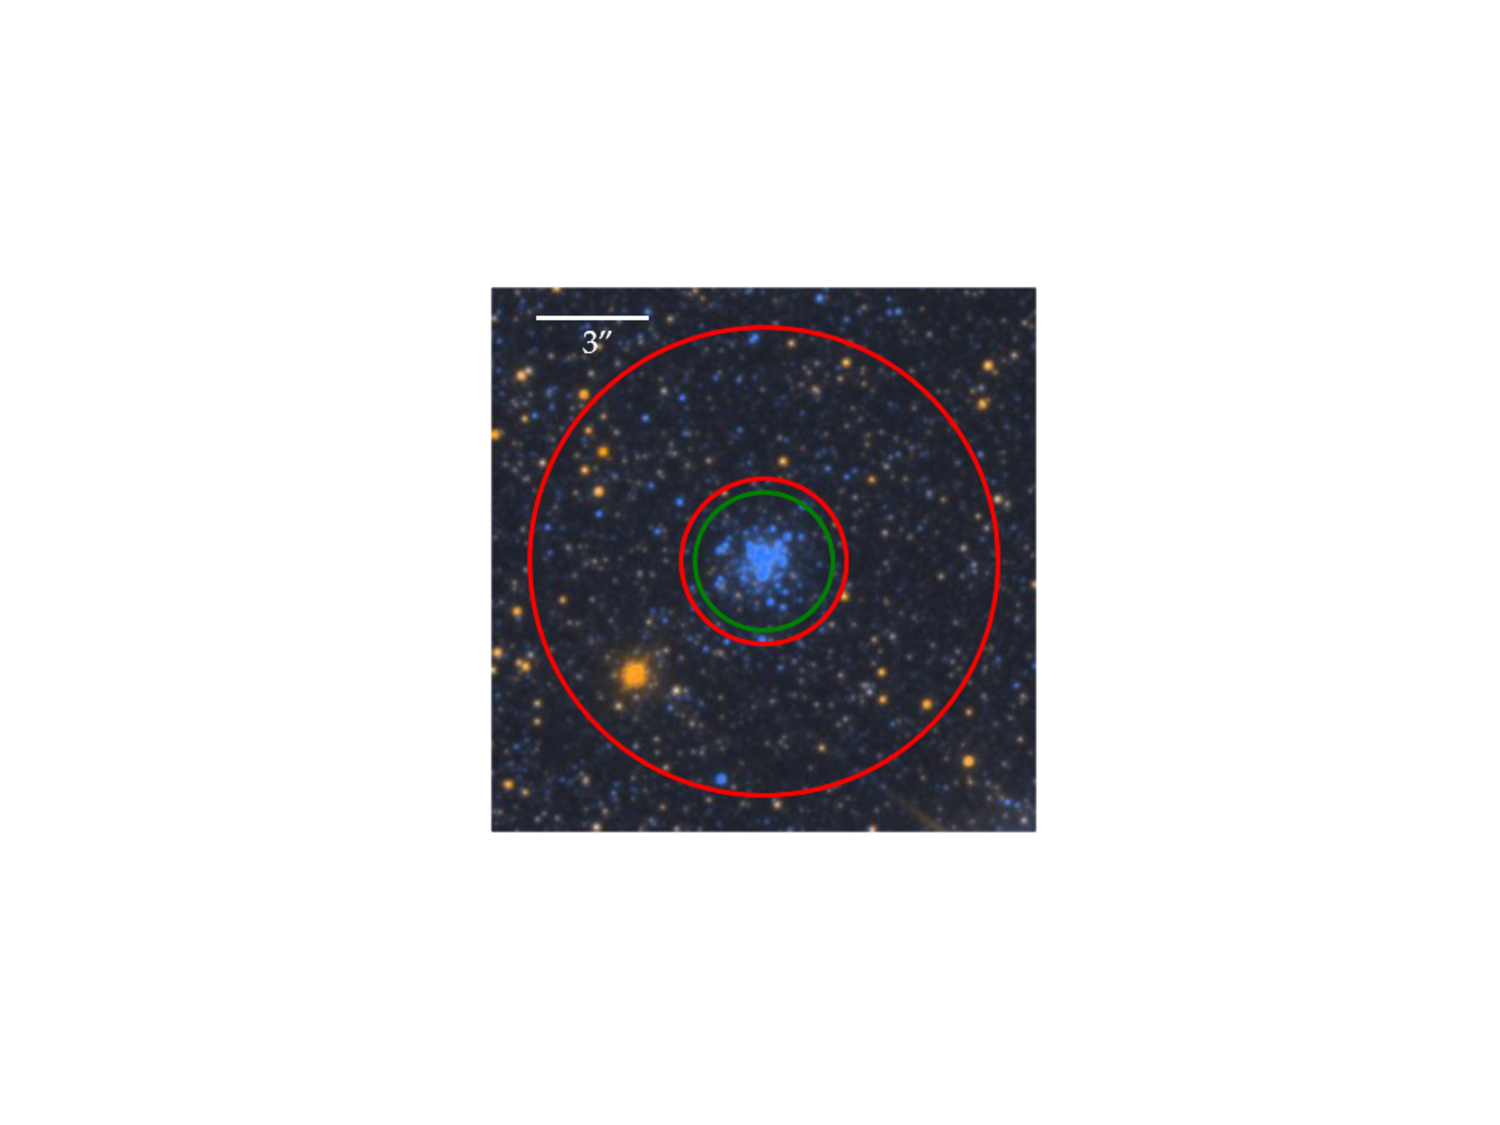
\includegraphics[trim=5cm 5cm 5cm 5cm, clip=True, scale=0.6]{ap81_rad.pdf} 
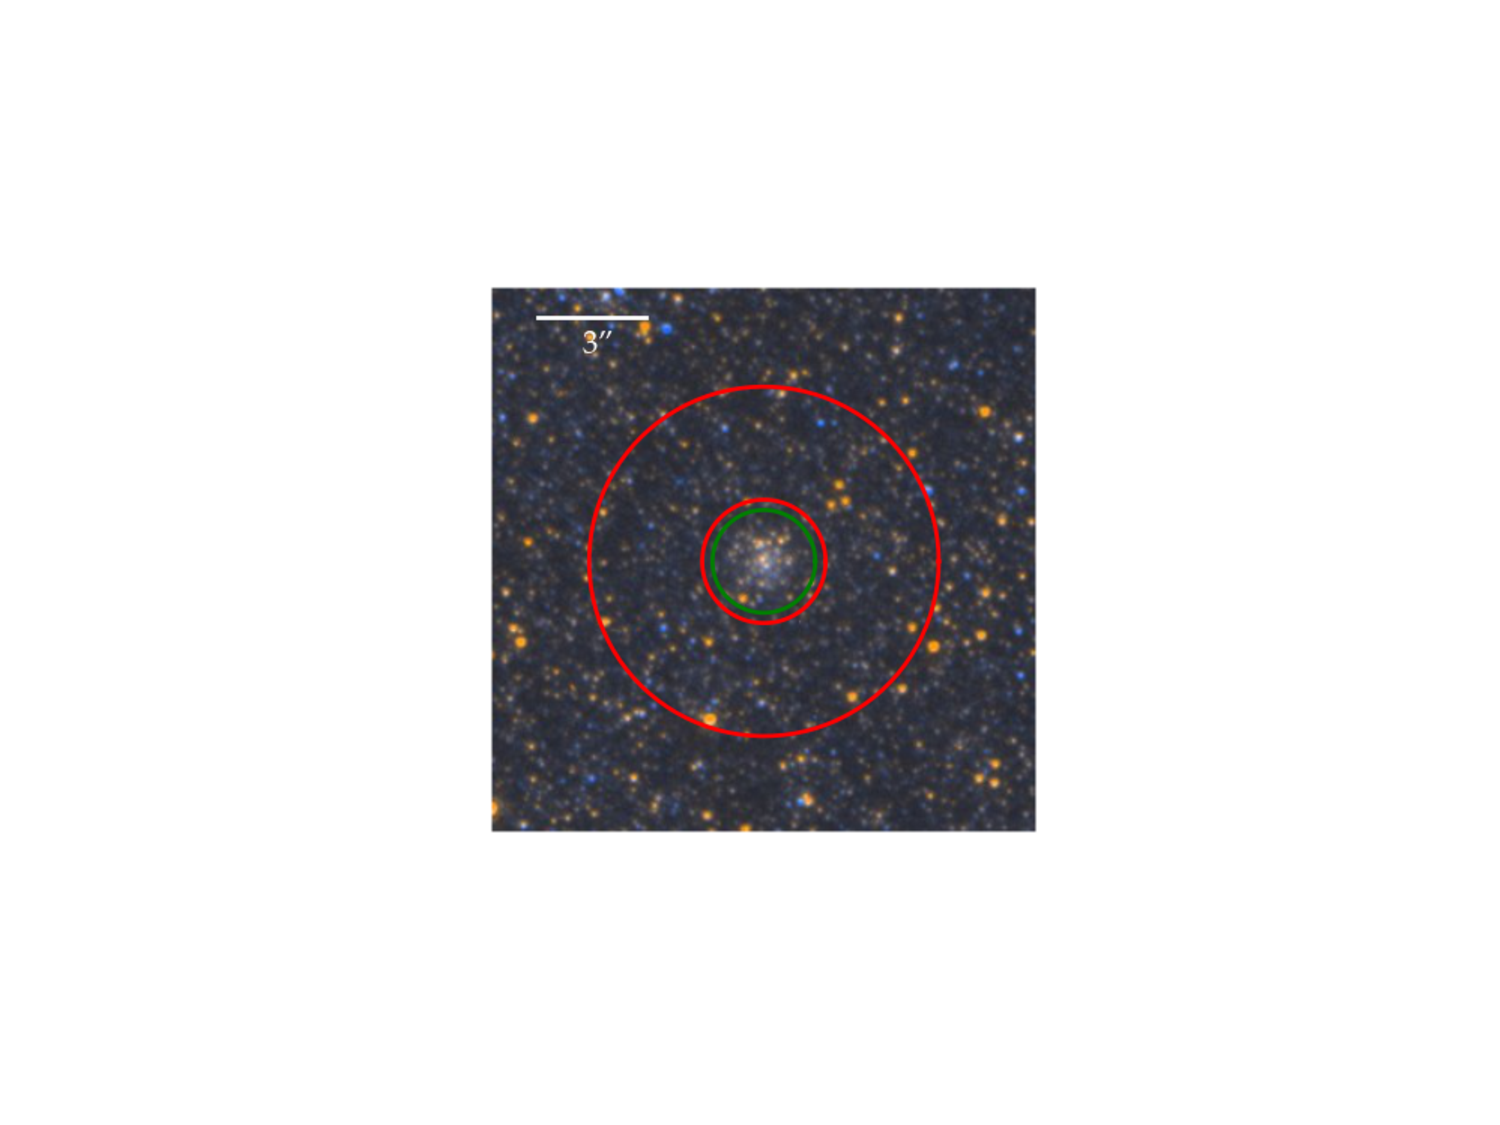
\includegraphics[trim=6cm 5cm 5cm 5cm, clip=True, scale=0.6]{ap71_rad.pdf}}}
\caption{Two example HST/ACS optical images of clusters in the PHAT sample.  AP81, a typical young cluster is shown in the left panel, and AP71, an older cluster is shown on the right panel.  The green circle represents the cluster's photometric aperture, and the red circles show the annulus within which the background is taken.  The clusters are clearly resolved into stars.  However, the stellar background is complex, which complicates both interpretation of the CMD and measurement of the integrated light.}
\label{fig:images}
\end{figure*}

\cite{Johnson15} defined circular apertures for each cluster which ranged from 0.7" (2.7 pc) to 6.4" (24.2 pc) in radius.  The apertures were chosen by first centroiding on the smoothed F475W image, then visually inspecting the curves of growth for each cluster.  Each cluster's aperture is set to be the point where the cluster light profile drops below the background noise.  This choice of aperture size allows the maximum possible cluster stars included while minimizing contamination from background sources.  The same aperture size was used in each filter.

Photometry for individual cluster stars was performed with DOLPHOT, which is a version of HSTPHOT with HST specific modules \citep{Dolphin00}.  We also generated a "background only" CMD, by extracting photometry from within an annulus from 1.2 - 3.4 $\times$ the aperture radius, covering 10 $\times$ the cluster's area.

In Figure~\ref{fig:images} we show two example images and CMDs of clusters in the PHAT sample.  With HST, the individual cluster stars can be readily resolved.


Artificial star tests (ASTs) were used to assess completeness and photometric bias within each cluster.  The ASTs were generated by inserting the PSF of each AST into the photometry for that cluster and then redoing the photometry with and without that AST, then measuring the stars' recovered properties in each optical filter.  50,000 artificial stars were created for each cluster, with the stars being distributed both spatially as a function of their light profile and uniformly on the CMD.  Since we had to generate over 150 million ASTs for the optical bands alone, adding the other four bands would have led to an exorbitant amount of computation time being spent on AST creation.

\begin{figure*}[!htbp]
\centering
\mbox{\subfigure{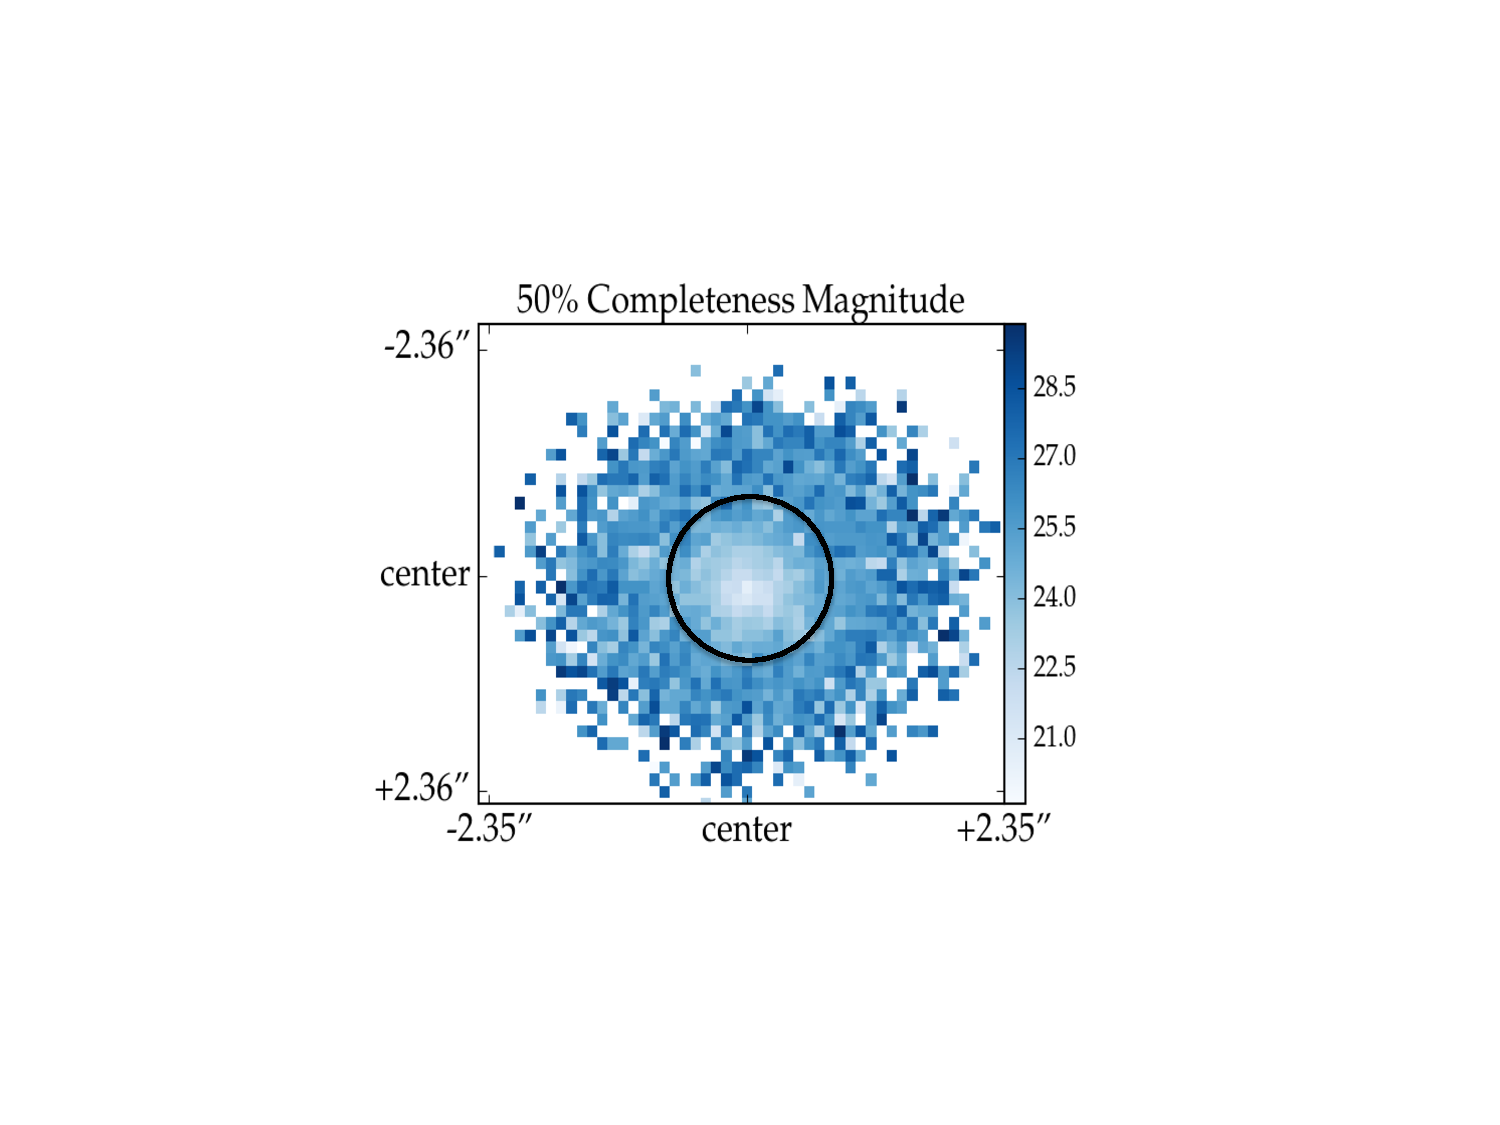
\includegraphics[trim=5cm 4cm 4cm 4cm, clip=True, scale=0.6]{ap2023_compmag1.pdf} 
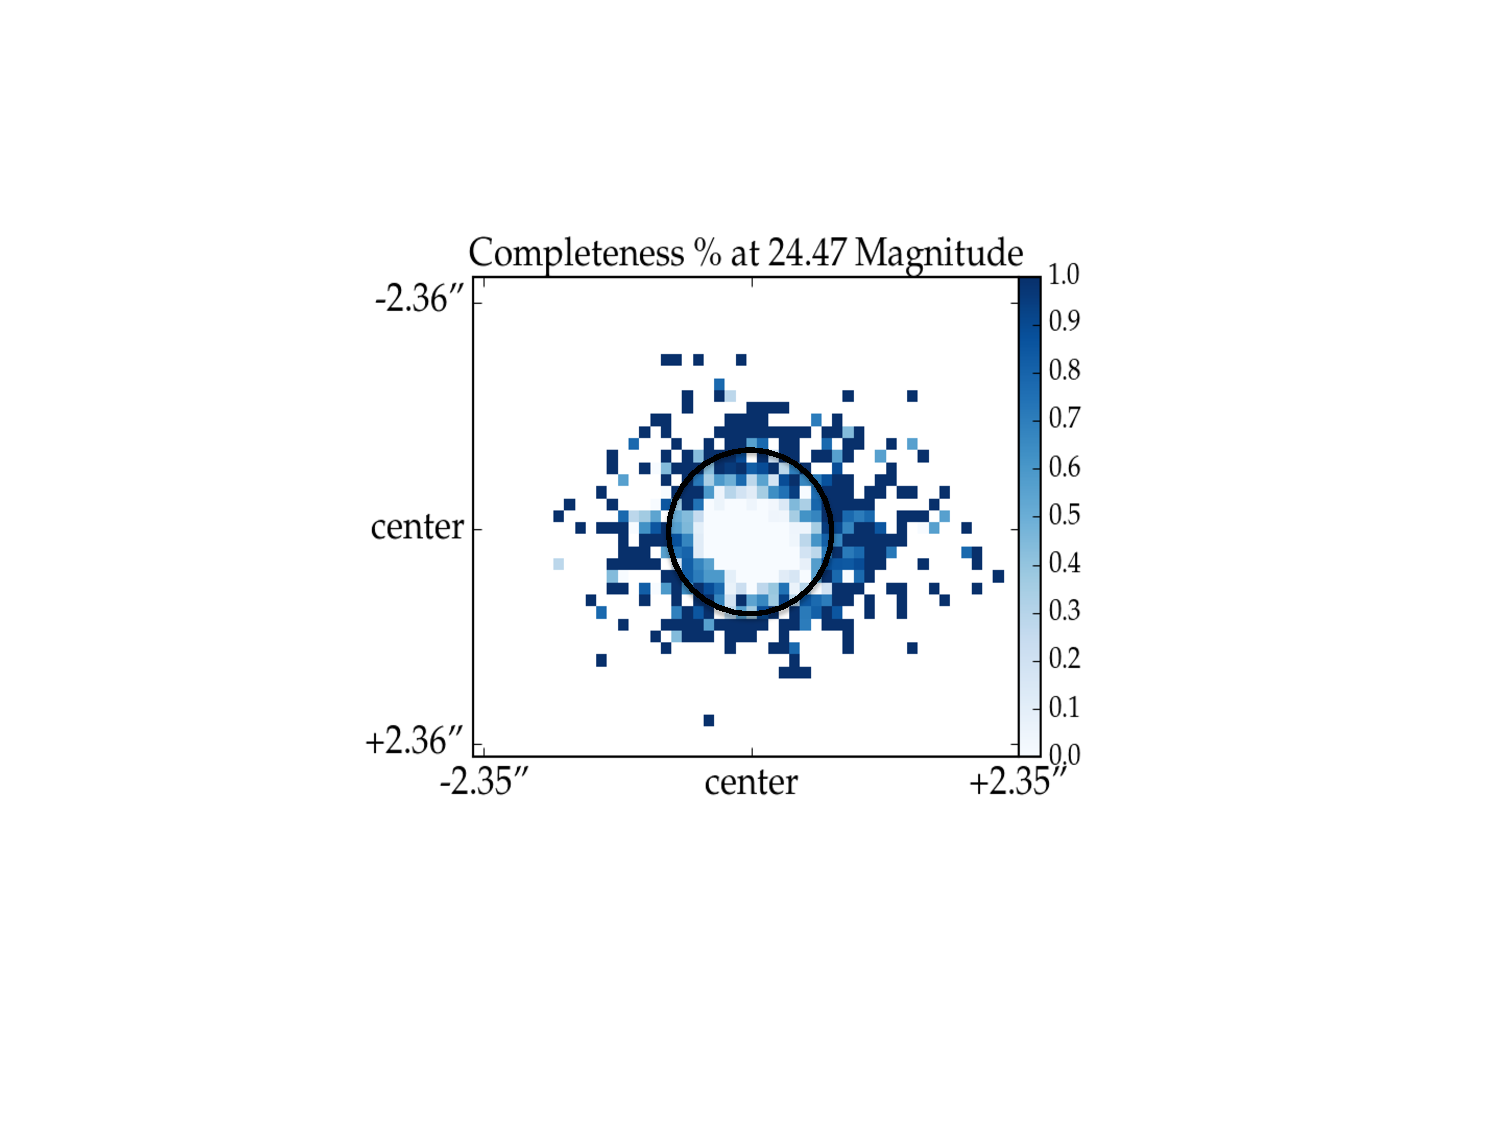
\includegraphics[trim=6cm 5cm 4cm 4cm, clip=True, scale=0.6]{ap2023_compmag2.pdf}}}
\caption{Spatial completeness maps for the dense stellar cluster AP2023.  The left panel shows the spatial distribution of the 50\% completeness magnitude and the right panel shows the completeness percentage at a fixed magnitude of 24.47 (corresponding to an absolute magnitude of 0).  The black circle shows the radial cut at 18 ${\rm mag/arcsec^2}$ in the F814W band which was used to remove photometry from stars within this radius that suffered from extreme crowding.  The overall completeness varies sharply with radius, changing from nearly zero completeness to \textgreater\ 80\% completeness over a change in radius of \textless\ 1".}
\label{fig:compmap}
\end{figure*}




\subsubsection{Crowding}\label{sec:crowding}

For some crowded clusters, crowding and blending of the central stars can significantly affect the CMD.  Inspecting the images and integrated light results show that this is a significant problem in the very crowded central regions of globular clusters.  This effect can be seen in Figure~\ref{fig:compmap}, which plots the spatial distribution of the 50\% completeness magnitude (left panel) and the completeness percentage at 24.47 magnitude (right panel, corresponding to an absolute magnitude of 0) for a crowded cluster.  The completeness percentage is clearly very low in the central region.  Due to this high crowding, in these low completeness regions, the small numbers of detected stars blend together and appear to be brighter than they are, and the majority of fainter stars are undetected.  When this happens, it creates a false "main sequence" on the CMD which can can produce a much younger fit in age than the actual cluster's age.  

We tried to limit the effects of severe central crowding by removing the central regions from the CMDs of the most crowded clusters and doing the MATCH analysis on the remaining stars.  Of the dense, older clusters in our sample, 118 have been previously observed by Caldwell et al (in prep).  Many of these are globular clusters that have severe crowding.  Caldwell et al (in prep) did a by-eye annulus fit to these clusters to attempt to define spatial regions that were not hampered by crowding effects.  We use his defined annuli for these clusters and only kept the stars  and ASTs that were were within the uncrowded annuli as defined by his by-eye annuli.

To extend this method to the entire cluster sample, we found the surface brightness that corresponded to the inner radii for the clusters in the Caldwell sample.  There are a few extremely crowded clusters that need a more strict surface brightness cut, but most of the clusters had a radial cut at about 18 ${\rm mag/arcsec^2}$ in the F814W band.  We adopted this as our surface brightness cut for the rest of the cluster sample.  We then found the corresponding radius for each cluster, and removed all stars both from the photometry and ASTs that are interior to this radius.  In Figure~\ref{fig:cmdonly} we show an example of the cluster CMD before (left panel) and after (right panel) the removal of interior stars.  For this cluster, the surface brightness cut removed mostly stars above F475W = 23.5, and the resulting best fit age changed from $log_{10} (t/yr)$ = 6.6 to 8.8.  



%\begin{figure}[ht!]
%   \begin{center}$
%     \begin{array}{cc}
%        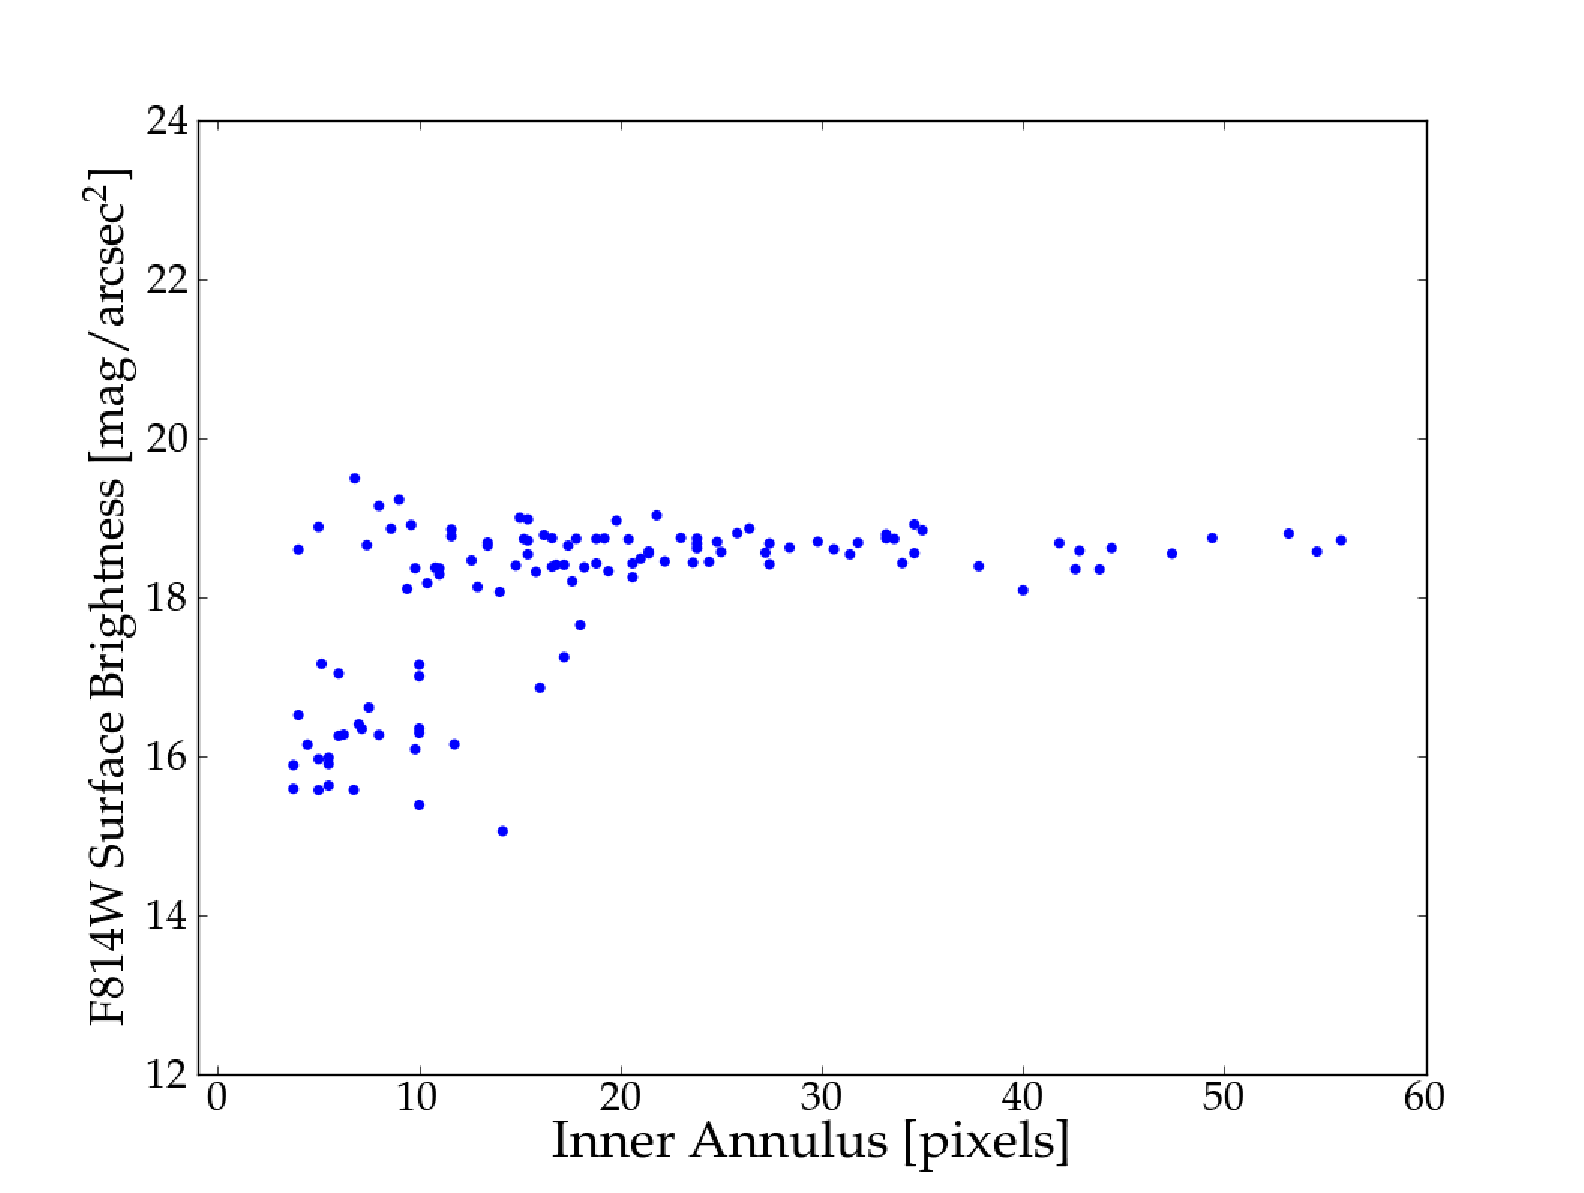
\includegraphics[trim=0.2cm 0.2cm 0.2cm 0.2cm, clip=True, scale=0.4]{SB_annulus.pdf} 
%    \end{array}$
% \end{center}
%  \caption{Inner pixel radius from Nelson vs surface brightness for globular clusters in his sample.}
%  \label{fig:SB}
%\end{figure}



This surface brightness cut affected 290 clusters.  Inclusion of this cut changed the ages of 25\% of these clusters, and eliminated the worst problems with crowding mimicking a young main sequence.  However, as we show below in Section~\ref{sec:broad}, there are a small number of crowded clusters that still appear to have artificially young ages.




\begin{figure*}[!htbp]
\centering
\mbox{\subfigure{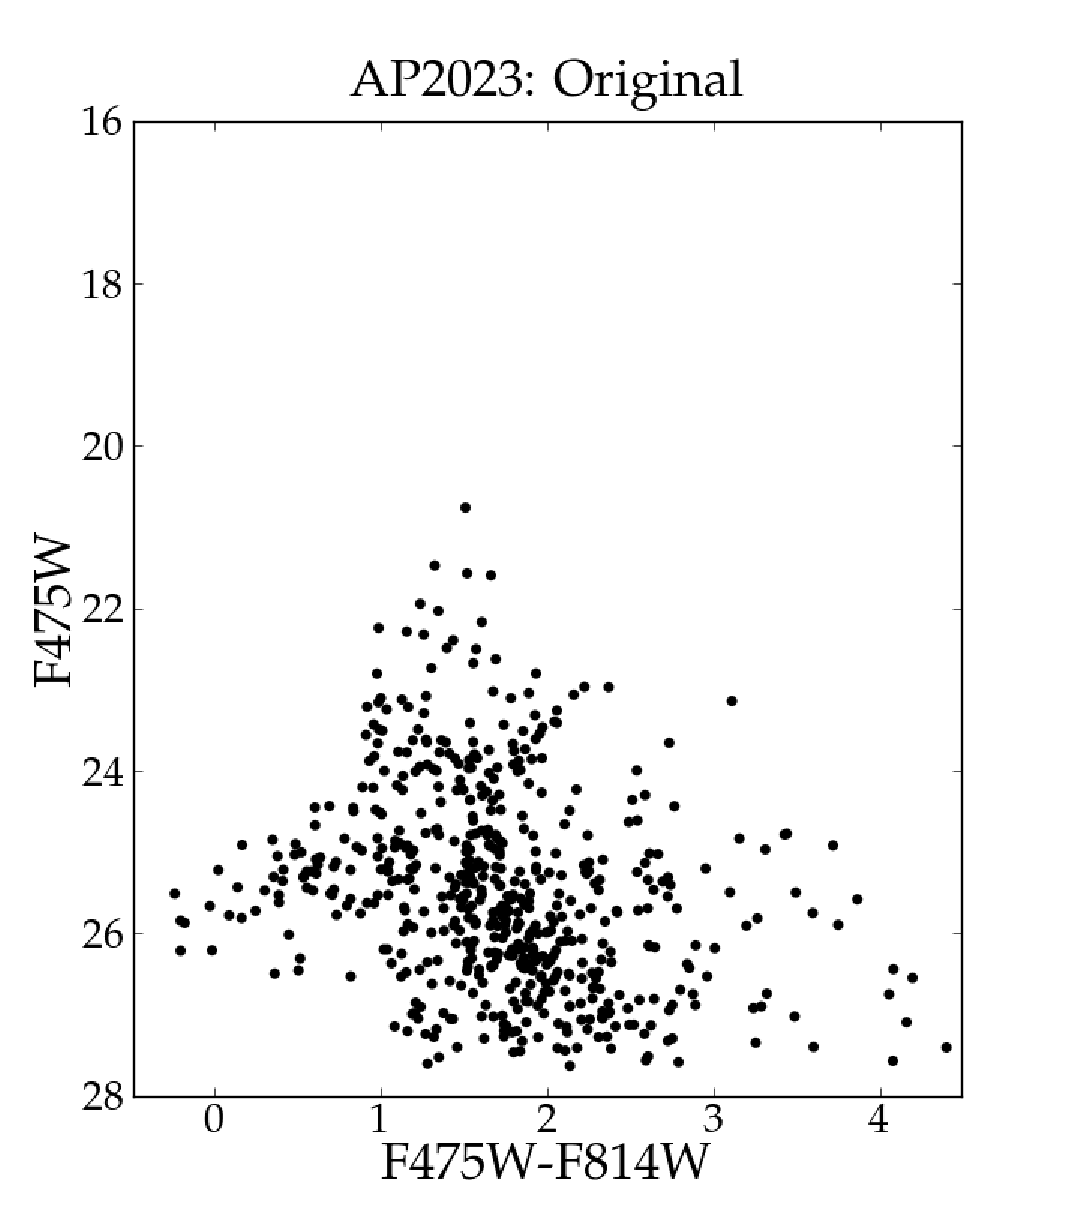
\includegraphics[trim=0.6cm 0.5cm 1.5cm 1cm, clip=True, scale=0.4]{ap2023_cmdonly_orig.pdf} 
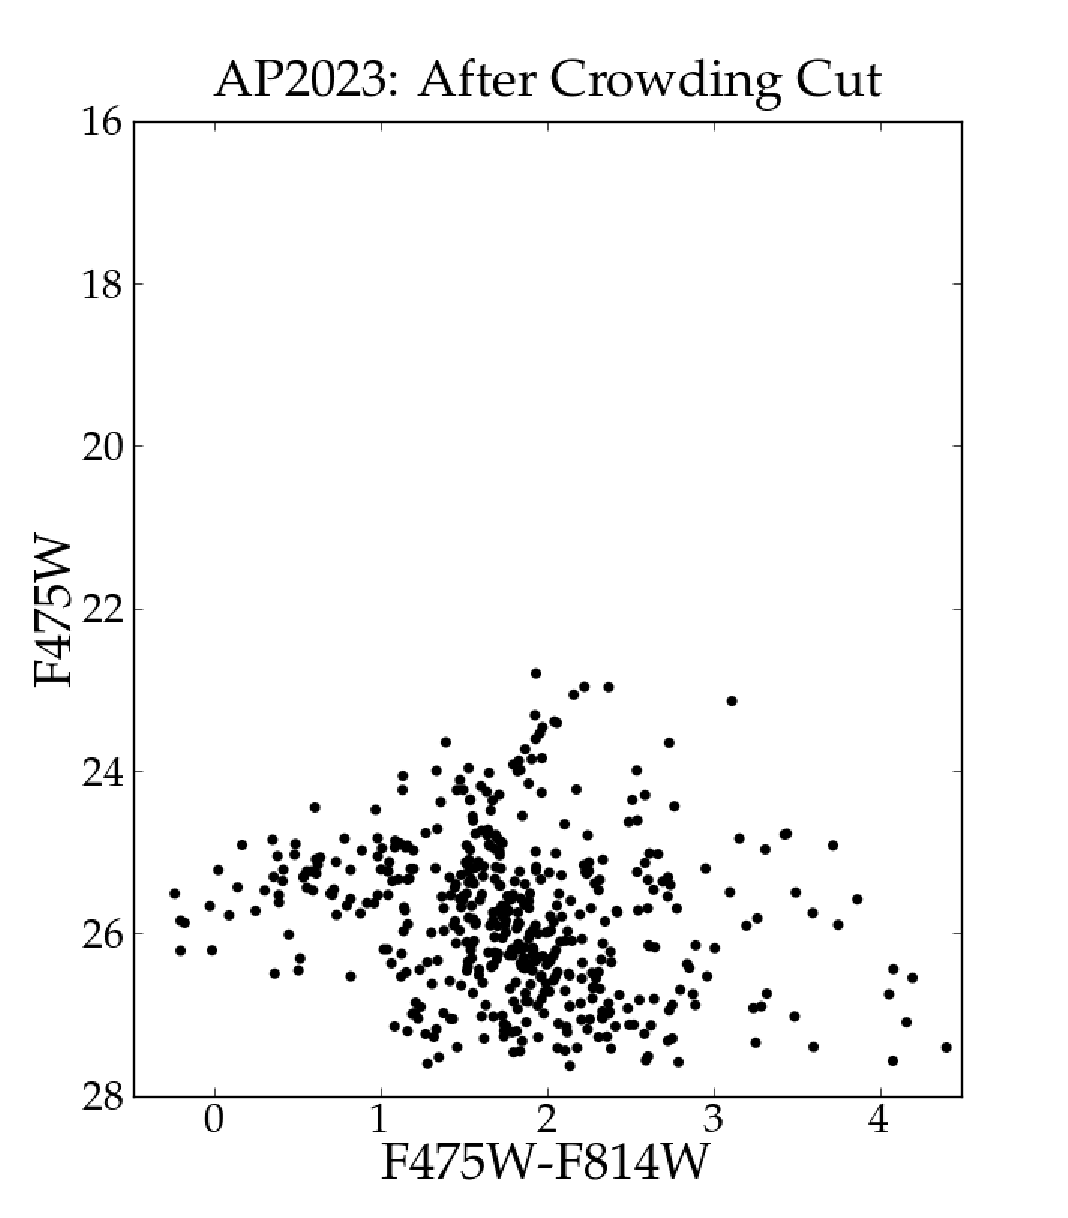
\includegraphics[trim=0.6cm 0.5cm 1.5cm 1cm, clip=True, scale=0.4]{ap2023_cmdonly_SB.pdf}}}

\caption{Original CMD for AP2023 (left panel) and after crowding cut using a surface brightness cutoff of 18 ${\rm mag/arcsec^2}$ (right panel).  This cut successfully eliminated bad photometry due to extreme crowding in the center of the cluster, leaving a CMD that shows a clear blue horizontal branch, characteristic of old metal poor globular clusters.}
\label{fig:cmdonly}
\end{figure*}




\subsection{Cluster Photometry:  Integrated Photometry}\label{sec:int phot}

For integrated photometry, \cite{Johnson15} performed integrated aperture photometry for each cluster in each of the six PHAT filters, using the apertures described in Section~\ref{sec:phot} for both the clusters and the background.  The background annulus for each cluster was divided into ten equal area annuli, and the integrated flux was measured in each.  To avoid sources that are not representative of typical background sources, two sigma outliers were rejected.  The mean flux of the non-rejected annuli are used as the background flux level, which is subtracted from the flux within the cluster aperture.  A signal over the background of at least 3 was set to be the minimum detection threshold in a given band.  For consistency with the stellar photometry, all flux measurements used the Vega magnitude system as reference, and the magnitudes were kept in the native HST filters.  A complete description of how the integrated cluster photometry was done can be found in Section 4 of \cite{Johnson12}.  

Associated measurement uncertainties are lower than 0.2 magnitudes for most clusters.  Uncertainties in the background represent the largest source of uncertainty in the integrated photometric measurements.  Background uncertainties are calculated from the standard deviation of all the non-rejected annuli used in the background flux measurement.  To determine how much light falls outside the aperture, radial flux profiles are fit to each cluster, and the resulting fits are used to make aperture corrections.  Based on synthetic cluster tests, between 0.1 - 0.3 mag of light is lost from each cluster that is outside the aperture.  Aperture corrections are made by fitting a \cite{King62} profile to the cluster light and extrapolating out past the aperture.  Uncertainties in the measured aperture flux are less than 0.01 magnitudes.  


\section{Determining Cluster Properties} \label{sec:properties}
In this paper we use two methods for determining cluster properties.  The first method is modeling the CMD fitting of the individual resolved stars in each cluster.  The second is fitting the integrated light (including upper limits) in six bandpasses to discrete probabilistic models.  In this section we describe each method and their corresponding strengths and limitations.

\subsection{CMD Fitting}\label{sec:cmd}
For Milky Way clusters and those in nearby galaxies (out to $\sim$ 2 Mpc), Modeling the CMD of the clusters' resolved stellar population provides the most robust determination of the clusters' properties.  CMD fitting allows us to take advantage of all the information in the main sequence and evolved stellar populations, including their colors, magnitudes, and relative numbers.  Modeling the entire CMD therefore provides the most accurate age, mass, and extinction determination for clusters with significant numbers of resolved stars above the completeness limit of the observations.
  
We performed CMD fitting to the resolved stars of each cluster using a modified version of the MATCH fitting program \citep{Dolphin02}, optimized for fitting a single age population plus a background model.  MATCH takes the following parameters as inputs:  IMF, binary fraction, extinction, distance, and stellar evolution library.  For a range of age and metallicity combinations, MATCH generates model CMDs using the given stellar evolution library for bins in CMD space.  Artificial star tests (ASTs) are used to model the completeness and photometric errors, which are then convolved with the model CMD.  The background is statistically modeled and added to the model CMD.  

The best fit age and extinction model is found using the minimum of the Poisson likelihood $\mathcal{L}$, since the number counts of stars in a CMD is Poisson distributed.  The mass is not a model parameter but is found by a normalization to the number of stars, assuming the appropriate mass-to-light ratio.  The goodness of fit parameter that comes out of the Poisson likelihood is used to infer the reported uncertainties.  The fit parameter is equal to -2 ln($\mathcal{L}$), meaning that the difference in the fit parameter of a given model relative to that of the best fit model goes as $\sigma^{2}$.  Thus, all fit values less than 1 away from the minimum fit value are within one standard deviation of the best fit.  This method produces a full probability distribution function (PDF) for each cluster.  When reporting uncertainties in a single parameter, we calculate the minimum and maximum values that are within one standard deviation of the best fit.

We ran each cluster through MATCH in the single stellar population mode.  We considered 36 age bins distributed in $log_{10} (t)$ between 6.6 and 10.1 with 0.1 dex spacing, and a single bin from 10.1 to 10.15 at the oldest ages.  Tests at finer age bins of 0.05 dex spacing showed no difference in results, and substantially longer computation times.  Since the disk of M31 has approximately solar-like metallicity \citep[e.g.,][] {Sanders12, Zurita12}, we chose to only fit around solar metallicity (-0.2 to 0.1 solar $Z_{\odot}$ with 0.1 dex spacing) to limit computation time.  This assumption is not valid for the small population of old, low metallicity clusters, but these clusters are well fit by the integrated light measurements.  We used a \citet{Kroupa01} IMF, along with a binary fraction of 0.35.  The extinction was allowed to vary from 0 to 3.0 in steps of 0.05.  The distance modulus used was 24.47 \citep{McConnachie05}.  We used the stellar evolution models from Padova \citep{Marigo08} with updated AGB tracks from \cite{Girardi10}.





%\begin{figure*}[!htbp]
%\centering
%\mbox{\subfigure{\includegraphics[trim=0.0in 0.2cm 0.2cm 0.2cm, clip=True,  scale=0.7]{ap1001_cmd.pdf}}}
%\\
%\mbox{\subfigure{\includegraphics[trim=0.0in 0.2cm 0.2cm 0.2cm, clip=True, scale=0.7]{ap1002_cmd.pdf}}}
%\caption{Examples of best fit isochrone from CMD fitting along with cluster stars (left panels) and background stars (right panel) for two clusters.}
%\label{fig:violin}
%\end{figure*}



\subsubsection{Reliability of CMD Fitting} \label{sec:synthetic}


\begin{figure*}[!htbp]
   \begin{center}$
      \begin{array}{cc}
         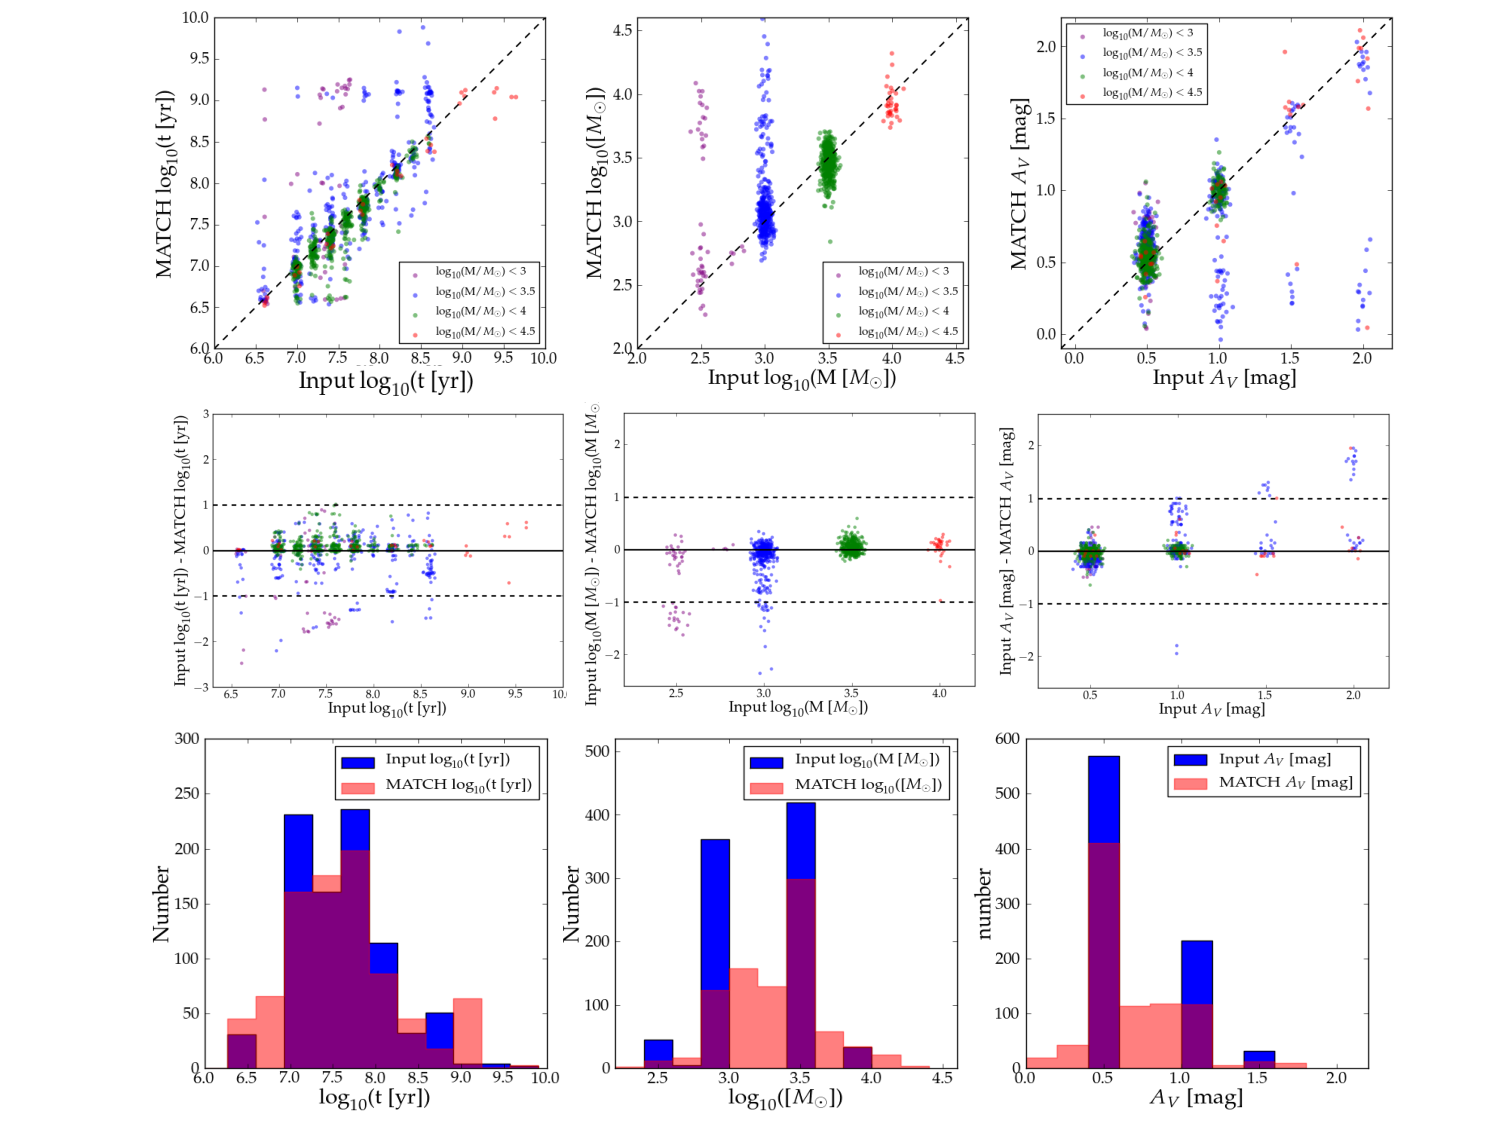
\includegraphics[trim=2.6cm 0.2cm 0.2cm 0cm, clip=True, width=7.8in]{syn_results528.pdf} 
      \end{array}$
   \end{center}
  \caption{Results from running 866 synthetic clusters through MATCH.  Top panels show each input parameter versus the Match recovered parameter, color-coded by input mass.  A small amount of Gaussian scatter was added for clarity to avoid overplotting points at discrete values of mass and age.  The middle panels show each input parameter versus the difference between input and recovered parameter, also color-coded by input mass.  The RMS deviation in $log_{10} (t)$ is 0.43 yr, the deviation in $log_{10} (M)$ is 0.34 $M_{\odot}$ and is 0.32 magnitudes in $A_{V}$.  Clusters above $10^3 M_{\odot}$ are recovered especially well.  The bottom panels show input and recovered histograms for each parameter.}
  \label{fig:synthetic}
\end{figure*}


To investigate how well MATCH recovers cluster properties, we tested MATCH's performance using a set of artificial clusters with known properties.  These synthetic clusters were created with a range of ages and masses, although we focused on ages less than 1 Gyr, where we expect to rely on CMD fitting rather than integrated light fitting.  These synthetic clusters were inserted into the PHAT images at various locations within the footprint, and then run through the photometry pipeline in a similar manner to the real clusters.  We also ran artificial stars for each of these synthetic clusters, in the same manner as the real clusters.

In Figure~\ref{fig:synthetic} we plot the input parameter ($x$-axis) vs the best fit result from MATCH ($y$-axis) for the 866 synthetic clusters.  The top panels are color coded by input mass.  A small amount of Gaussian scatter was added for clarity to avoid overplotting points at discrete values of mass and age.  There is good general agreement between the input and recovered parameters.  Fewer than 5\% of the best fit ages are more than 1 dex away from the input age, and only 12\% are more than half a dex away.  The RMS deviation in $log_{10} (t)$ is 0.43 yr.  The cluster masses are generally more accurately recovered, with only 4.4\% of best fit masses being more than 1 dex away from the input mass; 8.3\% are more than half a dex away.  The RMS deviation in $log_{10} (M)$ is 0.34 $M_{\odot}$ and 0.32 magnitudes in $A_{V}$.

To illustrate that failures in one parameter cause failures in another parameter, in Figure~\ref{fig:delta} we plot the difference between each parameter's input and recovered value.  In the top left panel we see that clusters with incorrect ages also tend to have incorrect extinctions.  The top right panel shows that failures in recovering age also tend to have failures in recovering mass.  The bottom shows that the same is true for mass and extinction.


\begin{figure*}[!htbp]
   \begin{center}$
     \begin{array}{cc}
        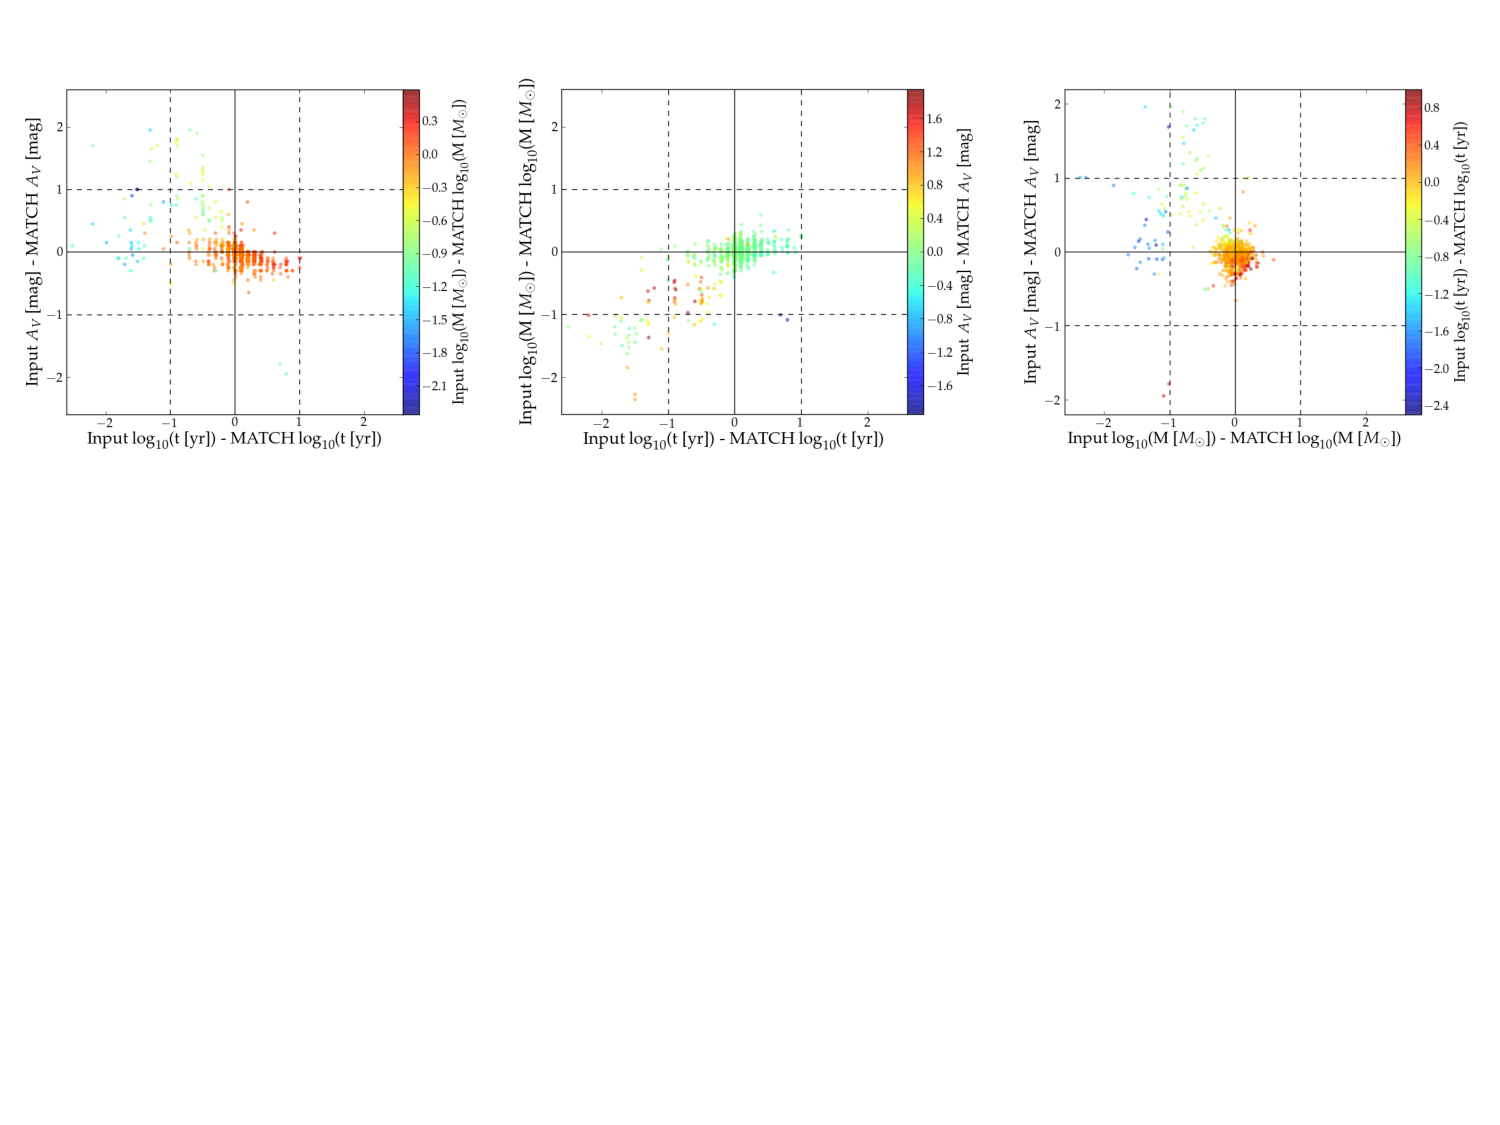
\includegraphics[trim=0cm 11cm 0cm 0cm, clip=True, width=7in]{delta1008.pdf} 
    \end{array}$
 \end{center}
\caption{The difference in input and recovered $log_{10} (t)$ versus the difference in input and recovered $log_{10} (M)$ for synthetic clusters (left panel).  The difference in input and recovered $log_{10} (t)$ versus the difference in input and recovered $A_{V}$ for synthetic clusters (middle panel).  The right panel shows the difference in input and recovered $log_{10} (M)$ versus the difference in input and recovered $A_{V}$.  It is clear that failures in one parameter correlate with failures in the other parameters.}
\label{fig:delta}
\end{figure*}




The failure cases are mostly confined to low mass, young clusters that have been fit as older clusters due to sparse main sequences.  In these clusters, there are not enough stars on the main sequence for MATCH to reliably derive a young age.  The MATCH results are generally very accurate for clusters that are at least $10^3 M_{\odot}$, since these clusters have enough of a main sequence to be properly fitted by the CMD fitting technique.  Looking at just these clusters, only 1\% had best fit ages more than 1 dex away from their input age, and only 9.7\% were more than 0.5 dex away.


\begin{figure}[ht!]
   \begin{center}$
     \begin{array}{cc}
        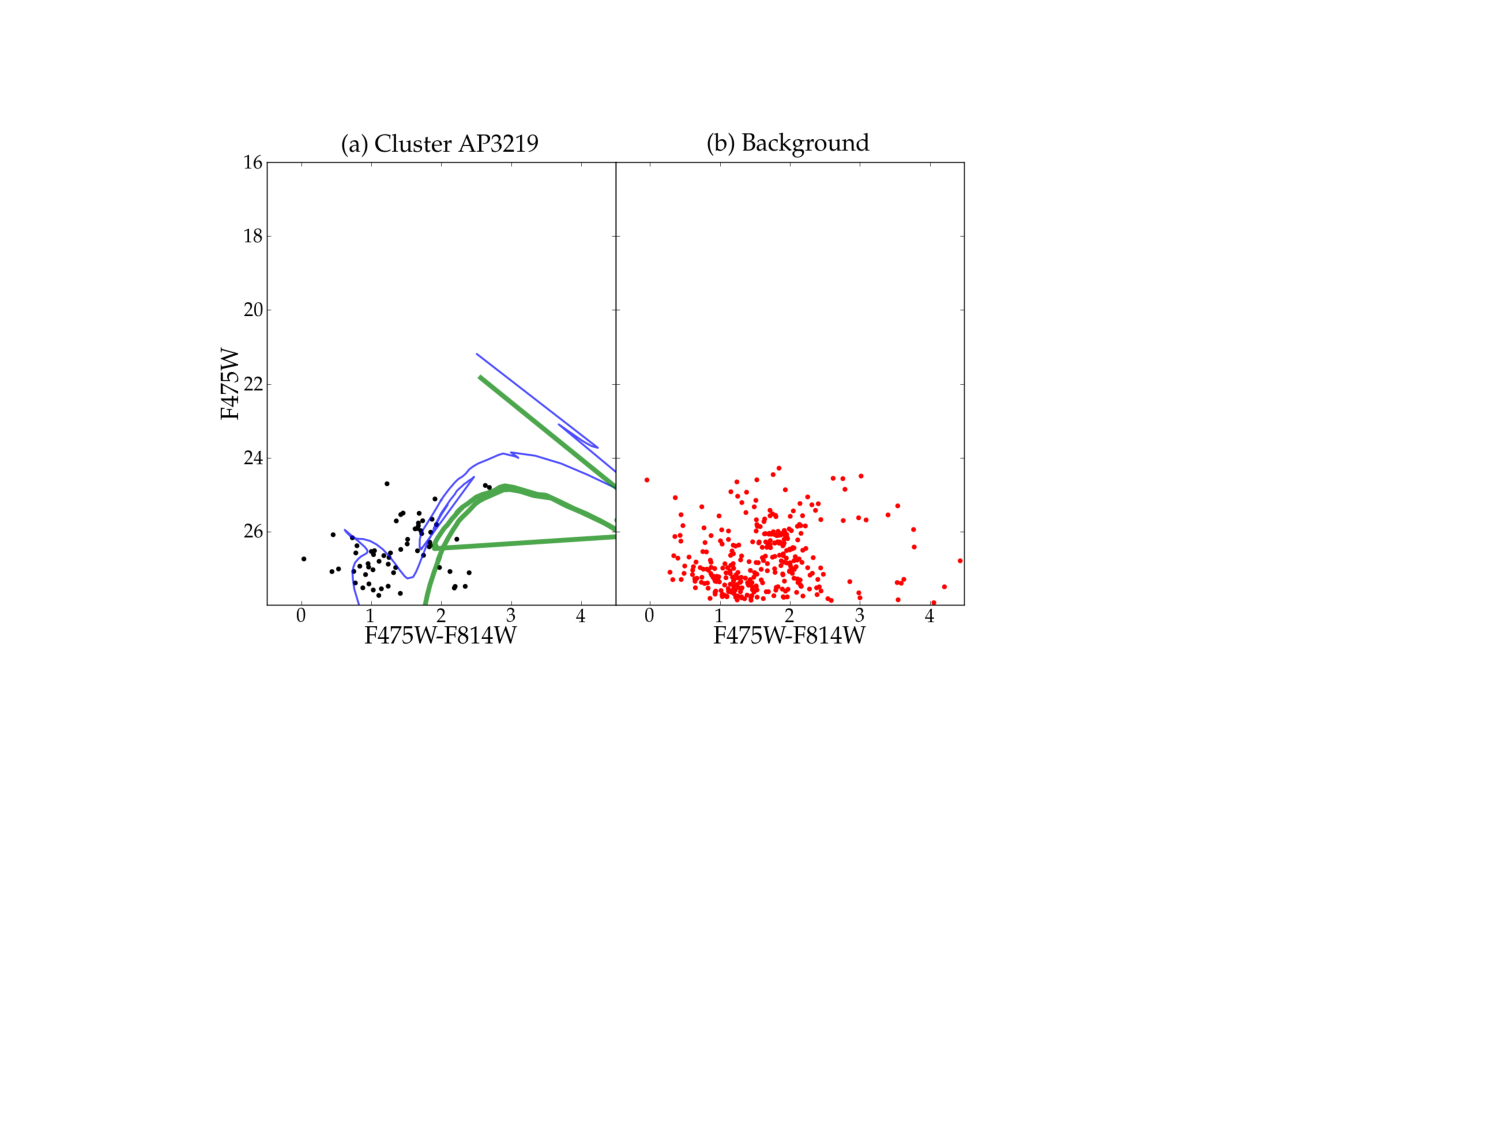
\includegraphics[trim=3.1cm 8.2cm 3.8cm 0.2cm, clip=True, scale=0.65]{ap3219_test.pdf} 
    \end{array}$
 \end{center}
  \caption{Color-magnitude diagram for PHAT cluster AP3219 in the left panel and the background population on the right panel.  The blue isochrone corresponds to the best fit age and extinction from CMD fitting, while the green isochrone corresponds to the expected age and extinction from integrated light fitting.}
  \label{fig:ap3219}
\end{figure}


When there are not enough cluster stars above our completeness limit (about 2-3 $M_{\odot}$), MATCH fits to the turnoff of the background stars, which is usually at 1 Gyr.  Figure~\ref{fig:ap3219} shows an example of a $10^{3.4} M_{\odot}$ cluster for which MATCH derived an age of 1 Gyr (blue isochrone), but the likely age from integrated light fitting (green isochrone) is much older.  The blue isochrone is clearly going through stars that are likely to be associated with the background.  We expect to see this feature in the PHAT cluster results for older and  very sparse clusters that do not have many stars above the completeness limit.
  


\subsection{Integrated Light Fitting}\label{sec:intlight}
Beyond $\sim$ 2 Mpc, individual cluster stars can no longer be resolved and integrated light measurements must be used to derive the clusters' properties.  More recent techniques that use integrated light now attempt to account for stochasticity by treating the mass function as a discrete distribution of stars \citep{Fouesneau10, Popescu10a, Deveikis08, daSilva12}.  These methods use discrete models generated from Monte Carlo simulations of clusters and compare the integrated properties of these to clusters integrated photometry to determine the clusters properties.  These methods perform better than traditional integrated light fitting.  However they still do not have the leverage available when modeling the distributions of individual resolved stars.

In this paper; we use the results from the Pegase.2n models that were described in \cite{Fouesneau14}, which was based on Pegase \citep{Fioc97}.  \cite{Fouesneau14} published properties for the \cite{Johnson12} "Year 1" PHAT cluster sample containing 601 clusters.  We now extend that probabilistic fitting of the integrated cluster photometry to the entire PHAT cluster sample.  This method uses discrete models made from Monte Carlo simulations of clusters from low (50 $M_{\odot}$) to high ($5 \times\ 10^{5} M_{\odot}$) masses, where stochastic sampling of the IMF is taken into account.  Above this mass the cluster's full mass function is being sampled, and continuous models are used instead.  The cluster spectral energy distributions (SEDs) in six filters are then compared to the discrete models and the full Bayesian posterior probability distributions are calculated in age-mass-extinction space, assuming power-law distributions of age and mass, and a uniform distribution of $A_{V}$ as priors.  

For our integrated light fits, model clusters ranged in age from 1 Myr to 20 Gyr, and their extinctions ranged from 0 to 3 $A_V$.  Metallicity was kept at solar for all discrete models, then a grid of metallicities from Z = 0.004 to 0.05 $Z_{\odot}$ was used for the continuous models, since these massive clusters are likely to be globular clusters with lower metallicities.  We marginalize over metallicity in the posterior probability distributions.  This technique is described in detail in \cite{Fouesneau10} and \cite{Fouesneau14}.  We adopt ages and masses for each cluster by calculating the mean of each PDF.  The uncertainties are calculated from the percentiles of the posterior distribution, and we report the $16^{th}$ and $84^{th}$ percentiles as our one sigma uncertainties. 


\begin{figure*}[!htbp]
   \begin{center}$
     \begin{array}{cc}
        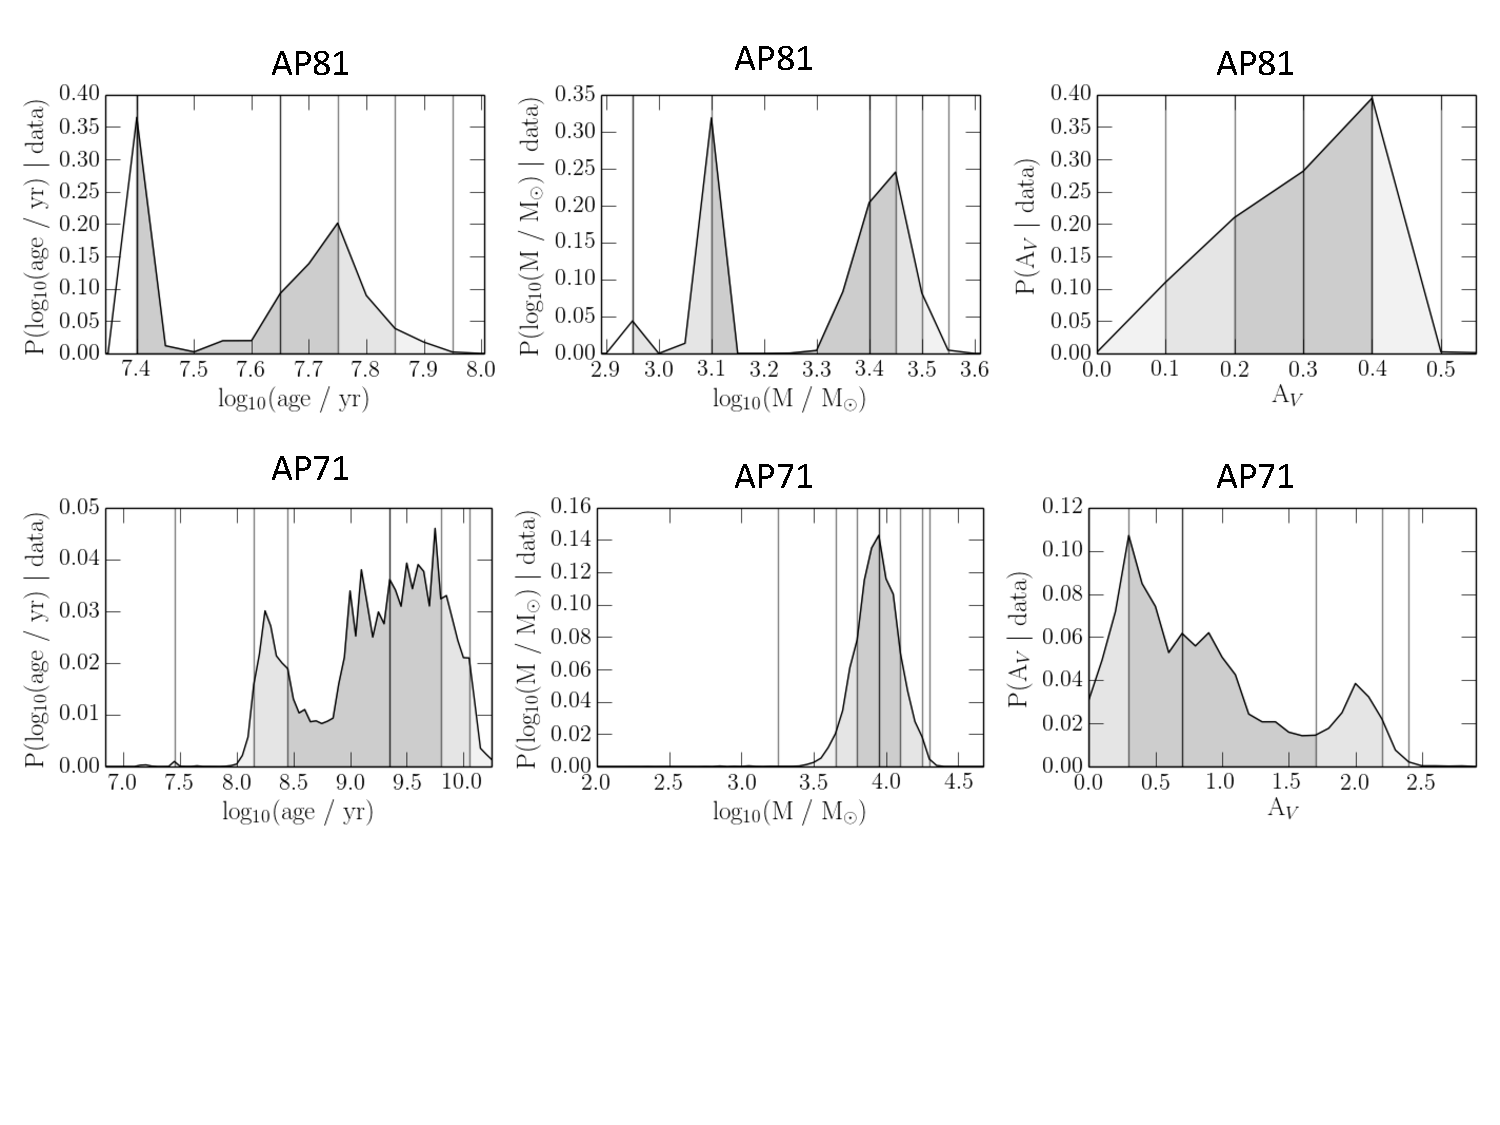
\includegraphics[trim=1cm 4cm 0.2cm 0.2cm, clip=True, scale=0.5]{int_uncertainties.pdf} 
    \end{array}$
 \end{center}
  \caption{Typical pdfs from the integrated light fitting showing the distribution of possible parameters.}
  \label{fig:ap3219}
\end{figure*}




\subsubsection{Reliability of Integrated Light Fitting}\label{sec:int_verify}

Even though discrete models do a much better job at predicting cluster colors in stochastic regimes, the problem of stochasticity still exists, especially when considering the issue of cluster membership.  If a background star is within the aperture, the integrated fit will include this star without considering whether there are enough other stars at the appropriate locations in IMF space to make the star a likely cluster member.  For many of these clusters, MATCH does not attempt to fit this bright star and treats it as a background star, since one would expect more stars slightly lower on the main sequence than are observed, if this truly were a cluster member.  Therefore, including a bright background star in the aperture may result in integrated light measurements that are too young for these clusters.  In Figure~\ref{fig:ap3320} we show the CMD of a cluster that has one bright star that is causing the integrated fit (green isochrone) to be much younger than the MATCH fit (blue isochrone). 

In addition, stochastic models are extremely sensitive to models of stellar evolution for rapidly evolving massive stars.  In stochastically sampled clusters, the integrated light is extremely sensitive to the presence of even one luminous star.  If stellar models do not predict the correct colors, magnitudes, and lifetimes of such stars, then the stochastic models cannot accurately capture the behavior of real clusters.  For example, stellar evolution models do not accurately predict the correct ratio of blue to red evolved core-Helium burning stars.  The models predict too few blue supergiants with respect to red supergiants, which leads to the integrated fitting predicting too young ages when a blue supergiant is present \citep{Dohm02, McQuinn11}.  This effect will be explored fully in Johnson et al (in prep).

\begin{figure}[ht!]
   \begin{center}$
     \begin{array}{cc}
        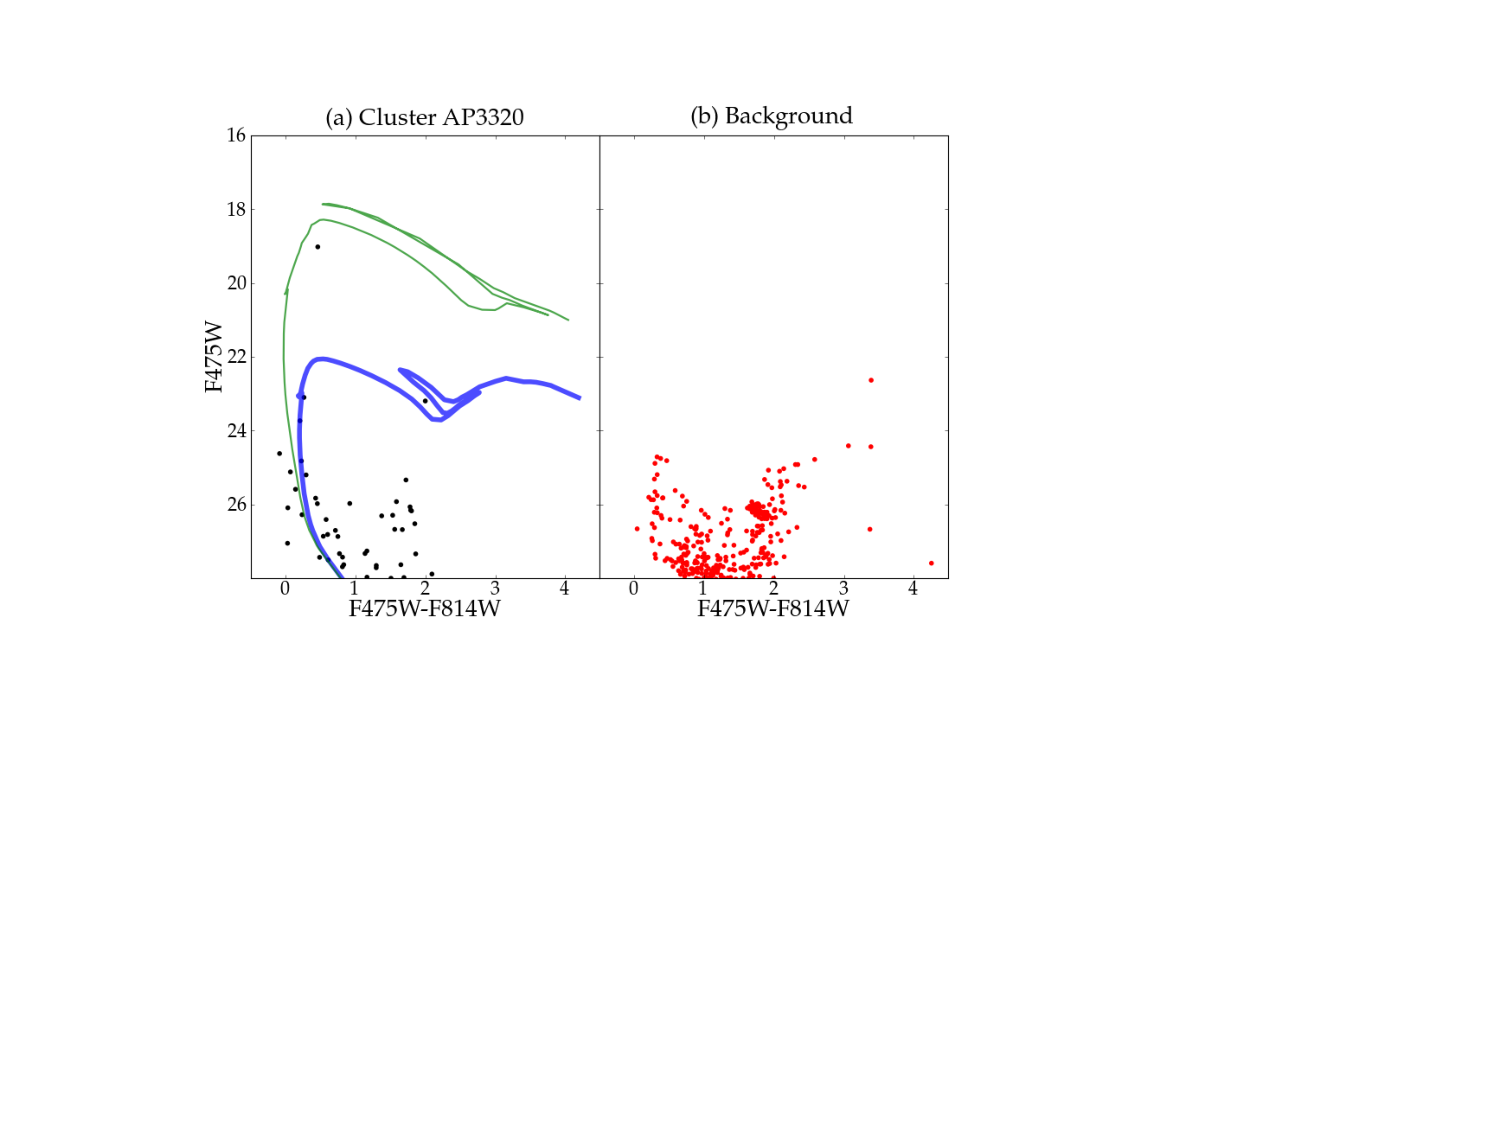
\includegraphics[trim=2.9cm 8.2cm 3.8cm 0.2cm, clip=True, scale=0.65]{ap3320_test.pdf} 
    \end{array}$
 \end{center}
  \caption{Color-magnitude diagram for PHAT cluster AP3320 in the left panel and the background population on the right panel.  The blue isochrone corresponds to the best fit age and extinction from CMD fitting, while the green isochrone corresponds to the expected age and extinction from integrated light fitting.}
  \label{fig:ap3320}
\end{figure}



\subsection{Merged Cluster Parameters}\label{sec:merged}
We have two completely independent techniques for determining the cluster parameters.  We can use these both for mutual verification and for identifying failure modes inherent in either technique.  We also use this comparison to decide which fiducial values to adopt for the age, mass, and extinction in subsequent analyses with this sample.


\subsubsection{Broad Sample-Wide Comparisons}\label{sec:broad}

{\emph {Ages:}}
In Figure~\ref{fig:int_match_comp} we compare the age that results from CMD fitting with MATCH to the age from integrated light fitting.  We account for uncertainties in their PDFs using Monte Carlo sampling of the PDF of each cluster 1000 times for both the MATCH and the integrated light PDFs. 

Overall there is a good agreement between the two methods.  60.71\% of the two ages are within 0.5 dex of each other, while 85.0\% are within 1 dex of each other.  The median one sigma uncertainty in age is 0.3 for MATCH, and 0.33 for the integrated light fitting, so there are comparable levels of reported uncertainty in the two methods.  The distribution is roughly symmetric about the 1:1 line, therefore there are no significant biases in either method with respect to each other.

While the overall agreement in age between the two methods is good, there are a few areas of differences.  Almost all the clusters whose integrated-fitted age is older than in MATCH, also have lower integrated extinctions, and vice versa.  Either the cluster is intrinsically red, thus older, or it is younger and heavily reddened.  

We also see a clear feature at 1 Gyr for the MATCH age results as described in Section~\ref{sec:synthetic}.  The vertical overdensity is a byproduct of CMD fitting failing when there are few cluster stars higher than the completeness limit.  This failure tends to occur when clusters are low mass, when the background is high, or when the main sequence turnoff is below the cluster completeness limit.  For our cluster sample, this means that the CMD ages will be less accurate for clusters older than a few hundred Myr.  


\begin{figure*}[!htbp]
\centering
\mbox{\subfigure{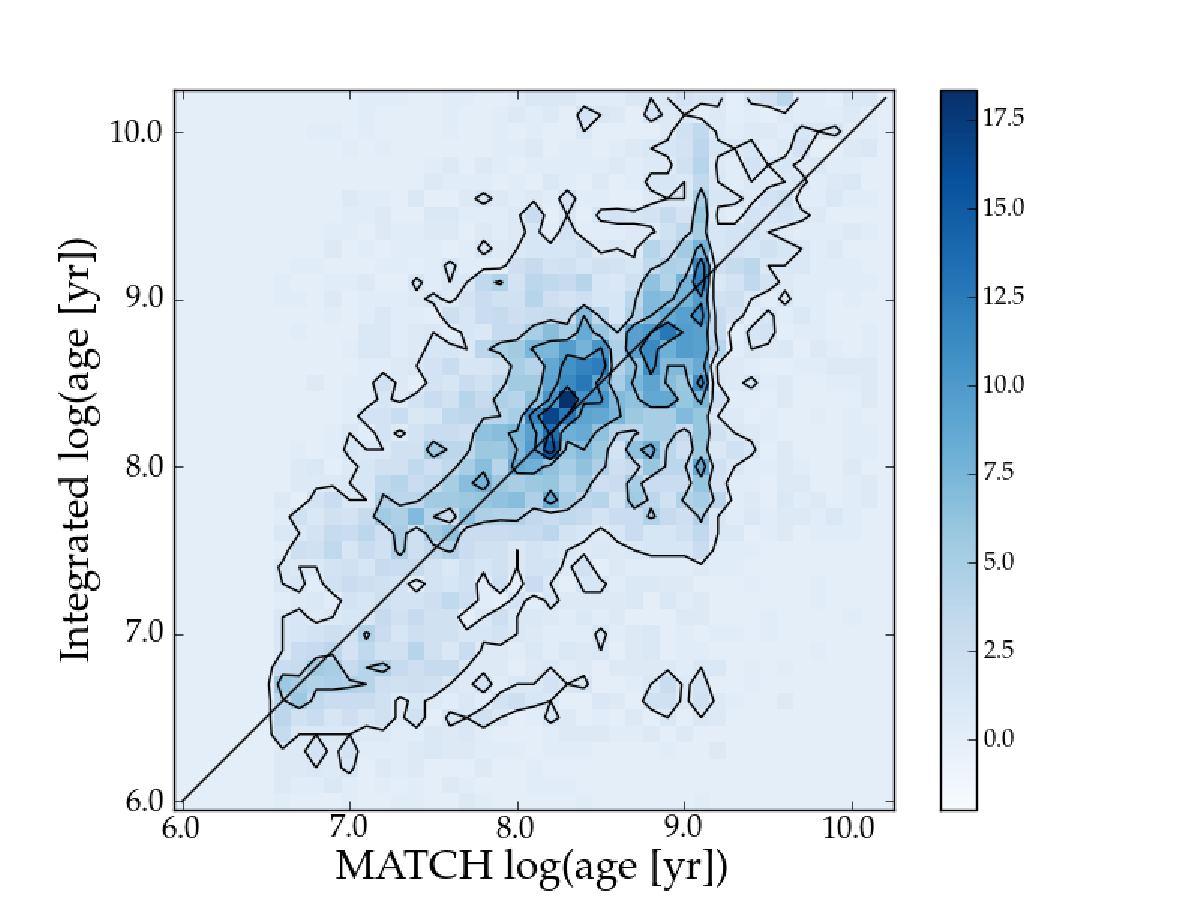
\includegraphics[trim=0.7cm 0.1cm 2.5cm 0.2cm, clip=True, scale=0.45]{plot_int_match_age.pdf} 
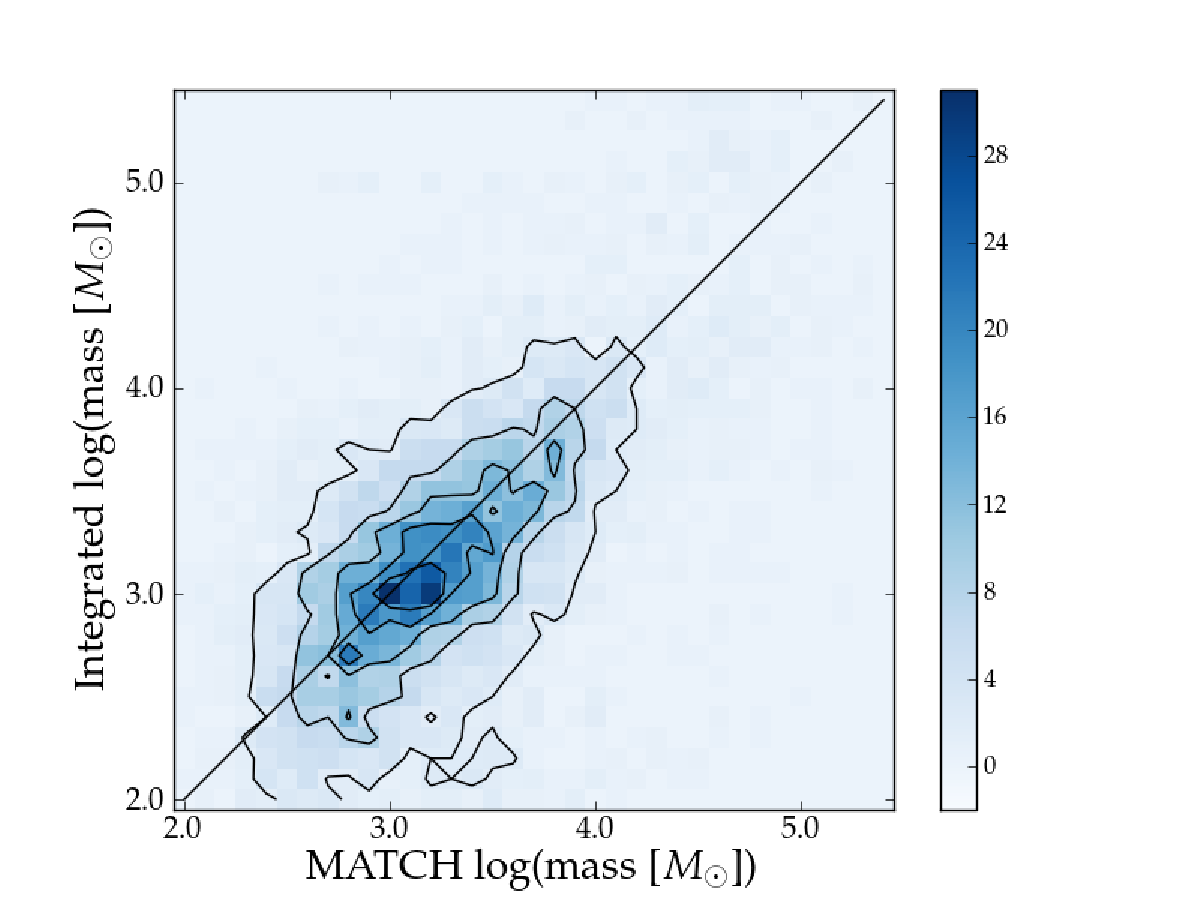
\includegraphics[trim=0.7cm 0.1cm 2.5cm 0.2cm, clip=True, scale=0.45]{plot_int_match_mass.pdf}}}
\\
\mbox{\subfigure{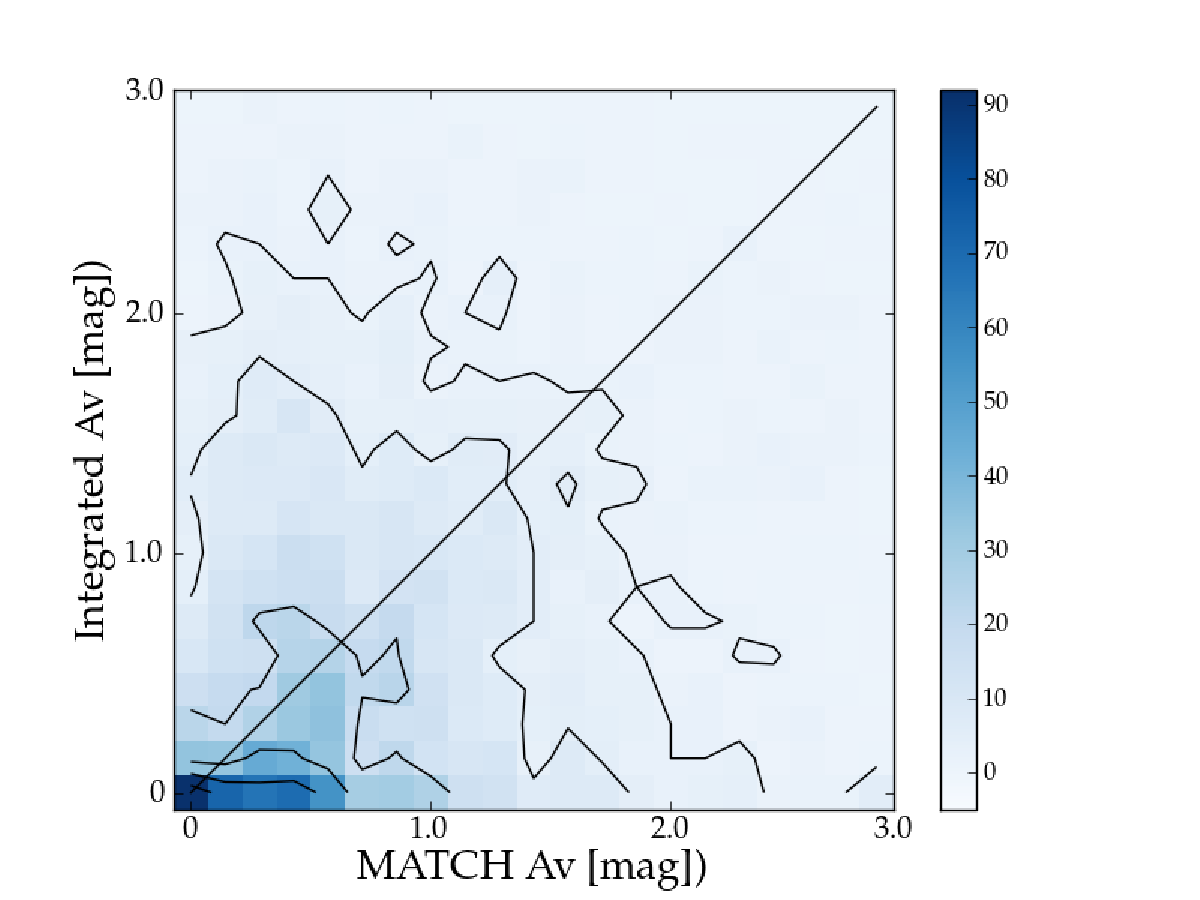
\includegraphics[trim=0.7cm 0.1cm 2.5cm 0.2cm, clip=True, scale=0.45]{plot_int_match_av.pdf}}}
\caption{Comparison of MATCH best fit results to integrated light expectation value.  Top left panel is age, top right is mass, bottom is $A_V$.  All plots have uncertainties in the PDFs incorporated by Monte Carlo sampling of the PDF.}
\label{fig:int_match_comp}
\end{figure*}


{\emph {Masses:}}
In Figure~\ref{fig:int_match_comp} we also plot the MATCH mass vs integrated mass.  The cluster masses from the two methods agree very well overall.  76.2\% of clusters have masses within 0.5 dex of each other, and 94.0\% of masses are within 1 dex.  

\subsubsection{Assessing Disagreements}\label{sec:disagree}
We know from earlier sections that neither method is expected to work well in all regimes.  There are three main categories of failure modes that might result in inaccurate fits.  First, even though we attempted to address crowding by applying a surface brightness cut and removing the centermost stars (as described in Section~\ref{sec:crowding}), there are about 100 clusters that are most likely Gyr or older clusters, based on their integrated colors and appearances, but that have crowding issues in the CMD, that have led MATCH to fit these clusters as younger.

The second situation that causes inaccurate fits is when a cluster has one or a few bright stars that contribute significantly to the integrated luminosity and drive the integrated light fits to younger ages, as seen in Section~\ref{sec:int_verify}.  We can get a sense of which clusters may experience this issue by calculating the cluster's "unresolved" magnitude and color, similar to what is done in \cite{Beerman12}.  Briefly, we derive the "unresolved" flux by subtracting flux from stars brighter than a cutoff magnitude from the integrated flux, which can then be converted into magnitudes and colors.  This correction diminishes the stochasticity while preserving a strong dependence of color on the cluster age.  However, because the integrated light measurements have already had background light subtracting off, subtracting off the flux of the brightest stars can leave a cluster with a negative flux, since we are "double subtracting" off the background component associated with the bright stars.  For our analysis here, we are only examining clusters whose integrated flux is greater than the "unresolved" flux.  To do a proper measurement of the "unresolved" flux, we would need to statistically add back the flux from background stars that are included in the aperture.  

To identify clusters that may be affected by background contamination, in Figure~\ref{fig:unres} we plot the MATCH age versus integrated age, where the size of the points represents the magnitude difference between the "unresolved" magnitudes and the integrated magnitudes.  We used a cutoff magnitude of F814W = -3 mag to compute the "unresolved" magnitudes, as in \cite{Beerman12}.  As expected, there is great variability in the magnitudes of young clusters, since these have been shown to suffer greatly from stochastic effects.  A high fraction of the clusters that the integrated light fits as young but MATCH identifies as old also show large variations in integrated -- "unresolved" magnitude relative to the other older clusters.  These are clusters where the MATCH ages are likely to be correct, but where a single bright foreground star has biased the integrated light results to young ages.


\begin{figure}[ht!]
   \begin{center}$
      \begin{array}{cc}
         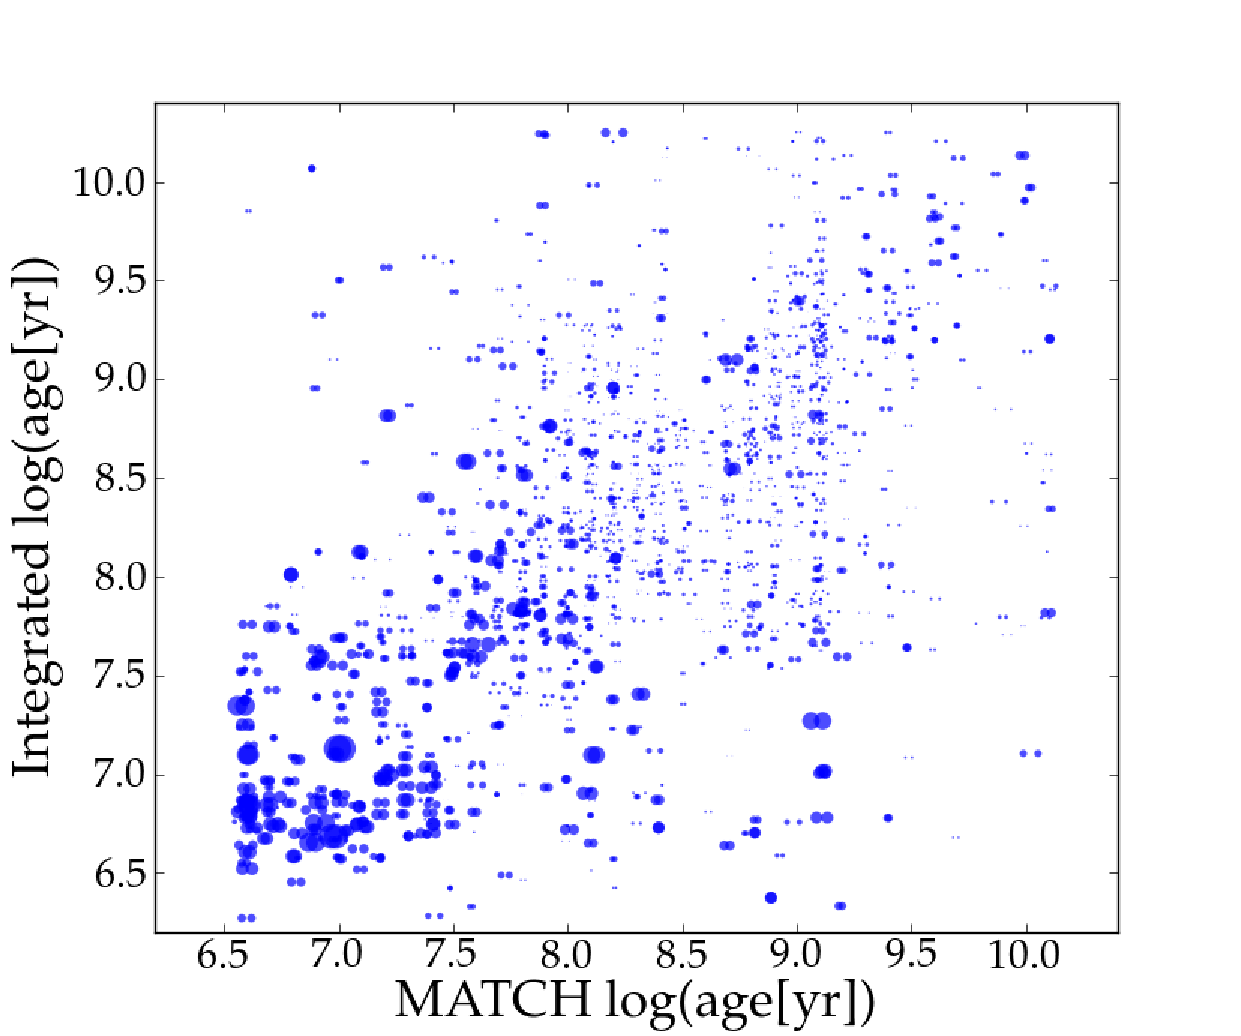
\includegraphics[trim=0.1cm 0.1cm 0.1cm 0.1cm, clip=True, scale=0.45]{age_unres475.pdf} 
      \end{array}$
   \end{center}
  \caption{MATCH versus integrated $log_{10} (t)$ where the size of the points represents the amount of variation in the cluster color when the brightest stars are removed.  A small amount of Gaussian scatter was added in the $x$-direction for clarity.  Older clusters show noticeably more stable colors.}
  \label{fig:unres}
\end{figure}



The third category of failure mode is when a cluster has too few resolved stars brighter than our completeness limit.  In these cases, MATCH will fit to the background stars, dominated by stars whose main sequence turn off is just above the completeness, since there are not enough cluster stars to provide significant age constraints, which was discussed in Section~\ref{sec:synthetic}.



\subsubsection{Assigning Parameters to the Cluster Sample}\label{sec:assign}

To carry out analyses of the PHAT cluster sample, we need to adopt a single "best" age, mass, and extinction for each cluster.  This step involves choosing the result from one of the two analysis methods.  We have argued that each method has a preferred regime, with CMD fitting expected to perform best at ages \textless\ 300 Myr where large numbers of turnoff stars are above the completeness limit.  Integrated light fits are expected to perform better at older ages where the effects of stochasticity are less, as shown in (Figure~\ref{fig:unres}, where the size of the points corresponds to the amount of variation in the cluster color when the brightest stars are removed).  However, we also know that neither method performs flawlessly, and have identified several possible failure modes.  

To pick the "best" fit for each cluster, we first adopt a default as MATCH providing the "best" fits for clusters \textless\ 300 Myr (in MATCH age), and integrated light as being the "best" fit for clusters older than this.  We visually inspect each cluster using its color cutout and optical images.  On each CMD we plot the isochrone corresponding to the best fit MATCH age and the isochrone for the expectation from the integrated light fit.  We looked through all of these and identified cases where the default best fit was a notably poorer match to the CMD, utilizing the image to help identify cases where crowding is a problem.  Clusters for which neither method produced an acceptable fit were flagged.  Additionally, clusters for which it was not clear which, method was correct (due to the issues in the previous section) were flagged.  Out of the 1649 young clusters, 91\% were acceptably fit by the default MATCH fit.  Out of the 1062 older clusters, 81\% were acceptably fit by the default integrated light.  Overall, only 1\% of the clusters were not well fit by either method, and about 10\% were not clear.  For these clusters which neither method is acceptable, or we are unsure which method represents the more accurate cluster parameters, we exclude them from the remaining analysis.  In Figure~\ref{fig:cmd_hist} we show the locations of the excluded clusters in CMD space.

**Need to discuss how excluding these clusters affects remaining analysis


\begin{figure}[!ht]
   \begin{center}$
      \begin{array}{cc}
         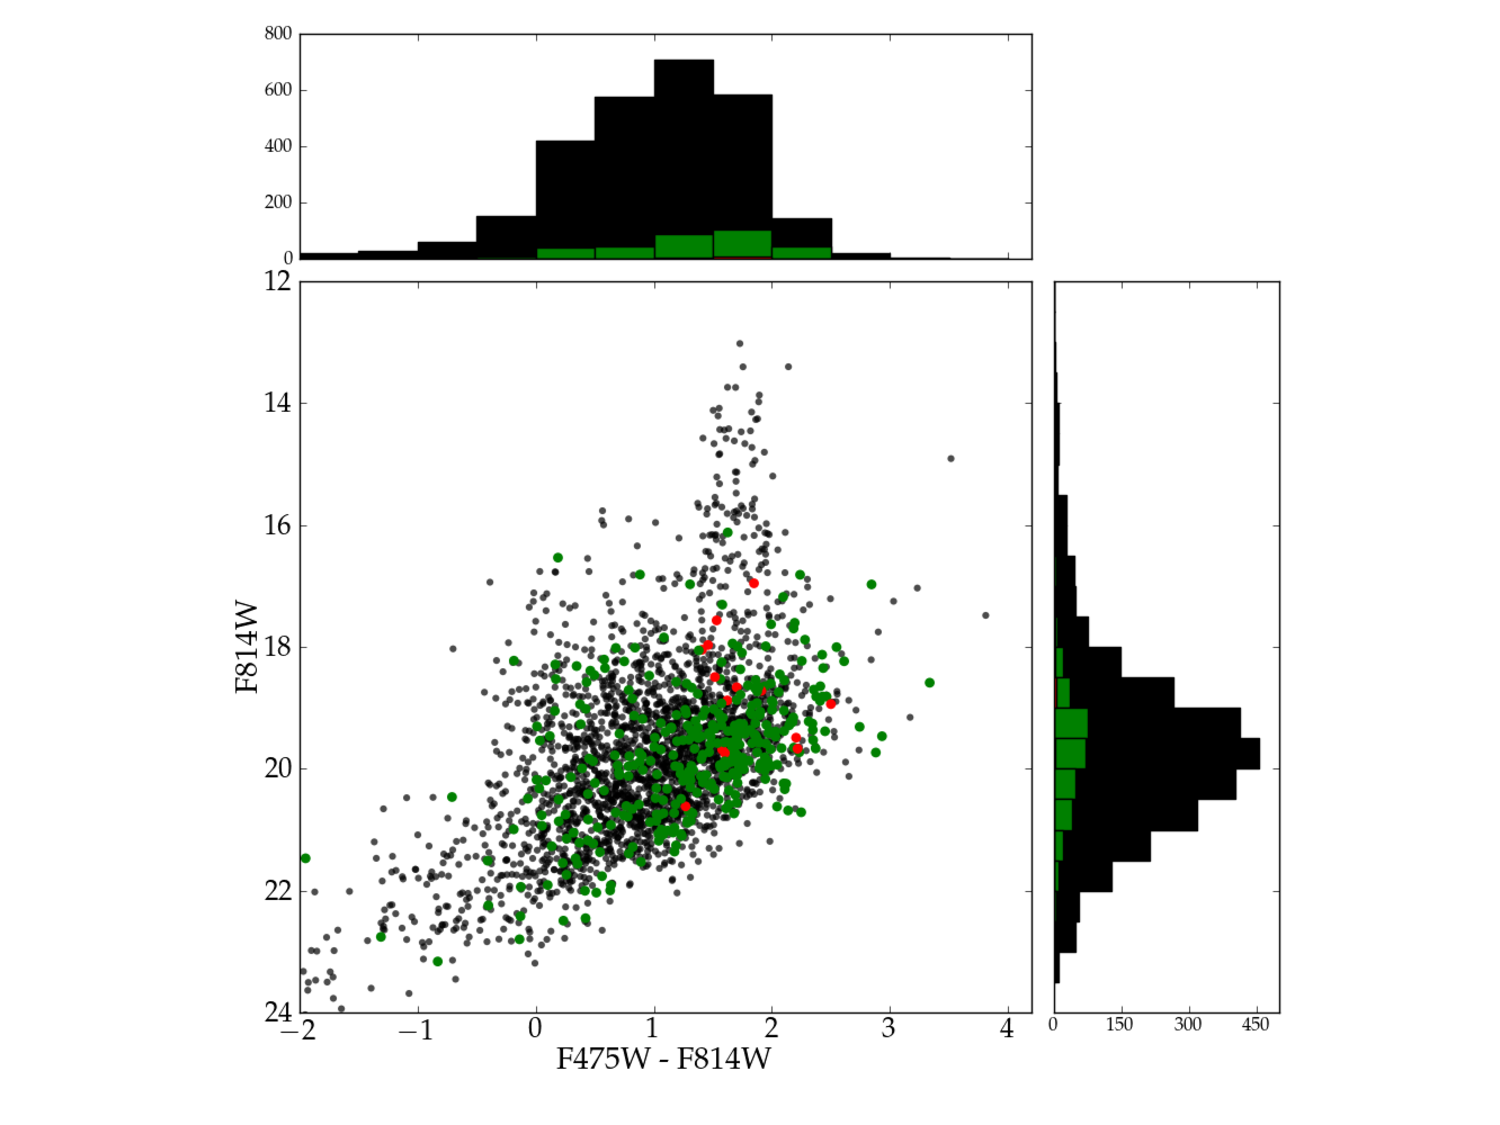
\includegraphics[trim=4cm 1cm 1cm 0.5cm, clip=True, scale=0.5]{plot_cmd_hist1.pdf} 
      \end{array}$
   \end{center}
  \caption{Color magnitude diagram for all clusters, where the red points represent clusters for which neither method produced an acceptable fit (1\% of the sample), and the green points represent clusters for which the best method was not clear (10\% of the sample).}
  \label{fig:cmd_hist}
\end{figure}


Our by-eye method of comparing fits resulted in a trusted value for the parameters of each cluster.  In Table~\ref{table} we show a stub table of the parameters for each cluster based on this evaluation.  A full table is shown in the Appendix.  These are the cluster parameters that we use for the rest of our analysis.


\begin{deluxetable*}{lccccccccccccc}
\centering
\tablewidth{0pt}
\tabletypesize{\scriptsize}
\setlength{\tabcolsep}{0.02in} 
\tablecaption{Cluster Parameters\label{table}}
\tablehead{
\colhead{}  & \multicolumn{3}{c}{CMD Best Fit Parameters\tablenotemark{b}}  &  \colhead{} 
& \multicolumn{3}{c}{Integrated Best Fit Parameters \tablenotemark{c}} &  \colhead{} 
& \colhead{} 
& \colhead{}  \\
\cline{2-4} \cline{6-8}  \\
\colhead{AP ID\tablenotemark{a}} & \colhead{$\log_{10}$($t$ [yr])}  & \colhead{$\log_{10}$($M [M_{\odot}$])} & \colhead{$A_V$ [mag]} &   \colhead{}  & \colhead{$\log_{10}$($t$ [yr])} 
& \colhead{$\log_{10}$($M [M_{\odot}$])}  & \colhead{$A_V$ [mag]} &  \colhead{}  & \colhead{Best\tablenotemark{d}} & \colhead{Flag\tablenotemark{e}} & \colhead{$\rm{R_{ap}}$\tablenotemark{f}}  & \colhead{$\rm{N_{stars}}$\tablenotemark{g}}  & \colhead{$\rm{N_{bg}}$\tablenotemark{h}}}
\startdata

AP1 & $8.80^{+0.00}_{-0.00}$ & $4.04^{+0.03}_{-0.03}$ & $0.05^{+0.10}_{-0.05}$ & & $8.97^{+0.05}_{-0.05}$ & $4.13^{+0.05}_{-0.05}$ & $0.08^{+0.09}_{-0.08}$ & & I & 0 & 2.19 & 408 & 229 \\ 
AP2 & $8.40^{+0.00}_{-0.00}$ & $3.98^{+0.00}_{-0.03}$ & $1.15^{+0.00}_{-0.05}$ & & $8.73^{+0.10}_{-0.07}$ & $3.52^{+0.07}_{-0.07}$ & $0.15^{+0.12}_{-0.15}$ & & I & 0 & 1.86 & 255 & 169 \\ 
AP3 & $8.80^{+0.00}_{-0.10}$ & $3.48^{+0.05}_{-0.00}$ & $0.00^{+0.30}_{-0.00}$ & & $8.57^{+0.08}_{-0.09}$ & $3.09^{+0.08}_{-0.07}$ & $0.11^{+0.13}_{-0.11}$ & & I & 0 & 1.95 & 197 & 113 \\ 




\enddata

\tablenotetext{a}{Andromeda Project ID \citep{Johnson15}}
\tablenotetext{b}{Best fit parameter results from CMD fitting using the MATCH package \citep{Dolphin02}.}
\tablenotetext{c}{Weighted mean of the PDF results from fitting the integrated light using Pegase.2n \citep{Fouesneau14}.}
\tablenotetext{d}{Method that produces the most accurate results.  The default is CMD fitting for clusters \textless\ 300 Myr and integrated fitting for clusters older than 300 Myr, but in individual cases the alternative method is adopted based on a by-eye quality check.}
\tablenotetext{e}{Flag set to 1 indicates best fit is not acceptable based on by eye quality check.}
\tablenotetext{f}{Aperture radius in arcseconds.}
\tablenotetext{g}{Number of stars in the cluster CMD.}
\tablenotetext{h}{Number of predicted background stars in the aperture.}



\end{deluxetable*}

In general the by-eye evaluation confirmed what we suspected from the plots in the previous sections.  Namely, that CMD fitting provides more robust parameter estimates for younger (\textless\ 300 Myr) clusters that still have multiple stars on their upper main sequence.  Integrated light determinations yield more accurate estimates for older clusters whose main sequence stars have already evolved.


\begin{figure}[ht!]
   \begin{center}$
      \begin{array}{cc}
         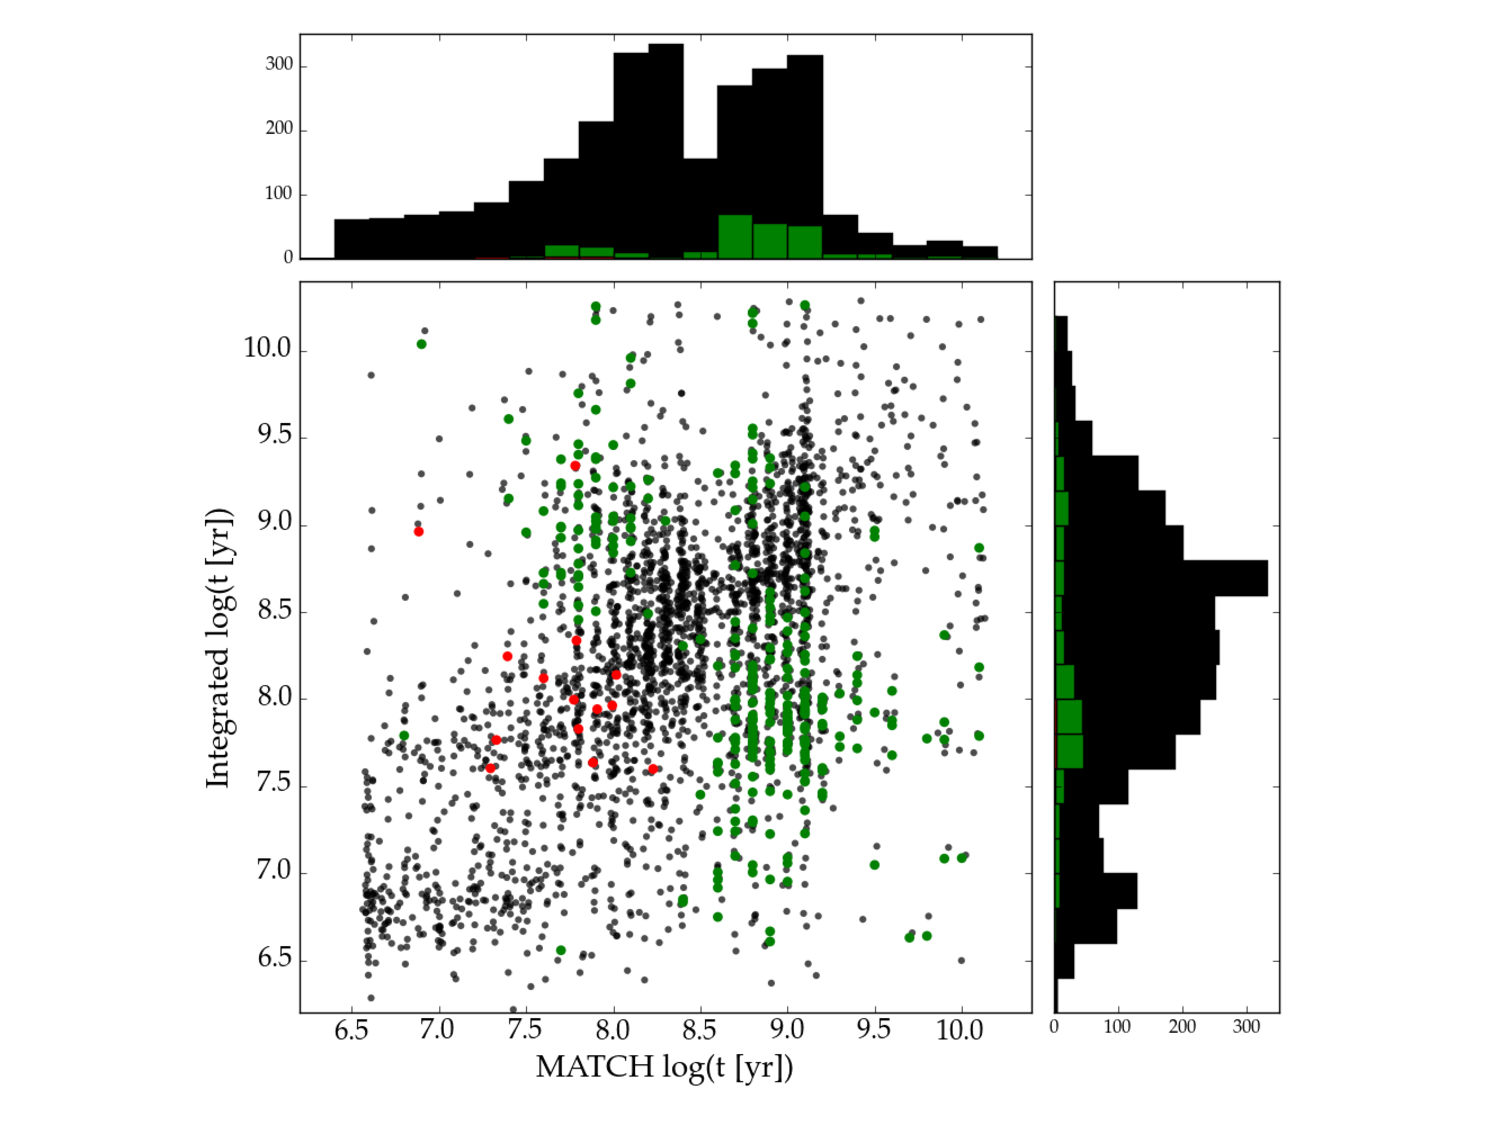
\includegraphics[trim=3.2cm 0.8cm 0.2cm 0.2cm, clip=True, scale=0.45]{hist_flag611.pdf} 
      \end{array}$
   \end{center}
  \caption{MATCH versus integrated $log_{10} (t)$ where flagged clusters with unacceptable fits in both methods are shown in red, and clusters where the non default fit is better are shown in green. Histograms on sides show distributions of each.  A small amount of Gaussian scatter was added in the $x$-direction for clarity.}
  \label{fig:flaghist}
\end{figure}

In Figure~\ref{fig:flaghist} we plot the MATCH ages vs the integrated ages, along with the projected histograms on each axis, where all clusters in the sample are plotted in black, and the clusters that were flagged as having neither the integrated nor the MATCH fits appear to be acceptable based on the CMD are shown in red.  The green points are those clusters for which the non default value is a better fit than the default fit (i.e., a young cluster whose integrated light fit is better than the MATCH fit).  From this, we can see that most clusters that were flagged had disagreements between their CMD and integrated ages.  In these cases the default method is not providing an accurate age for that cluster.  

The group of clusters that are likely older globulars that have crowding issues on their CMDs as described in Section~\ref{sec:crowding} can be seen in Figure~\ref{fig:flaghist} as the group of flagged clusters that have young MATCH ages and older integrated ages.  These clusters that have drastically younger integrated fits due to one bright possible background star are evident in the bottom right of Figure~\ref{fig:flaghist}, at older MATCH ages and younger integrated ages. 

We note that the histograms also show a larger fraction of clusters that have been flagged in the bins around a MATCH age of 1 Gyr, indicating poor fits likely due to MATCH fitting to the background stars when there are not enough cluster stars above our completeness limit, as described in Section~\ref{sec:synthetic}.

We can also investigate how the number of filters in which a cluster was detected correlates with the flagged clusters.  In Figure~\ref{fig:ndet} we show the integrated $log_{10} (M)$ versus the number of filter detections where all flagged clusters are shown in red.  A cluster was considered detected in a given passband if it had signal to noise (S/N) \textgreater\ 3 with respect to the variation in the background \citep{Johnson15}.  Naturally the more massive clusters tend to be detected in more filters.  It is interesting that clusters with detections in five and six filters have a larger percentage of flagged clusters than those with only three or four detections.   One possible explanation for this is that given more data points along with imperfect models may force some clusters into unusual places in the age-mass-extinction parameter space, where having fewer data points gives a greater degree of freedom to allow the models to fit the light in those filters.


\begin{figure}[ht!]
   \begin{center}$
      \begin{array}{cc}
         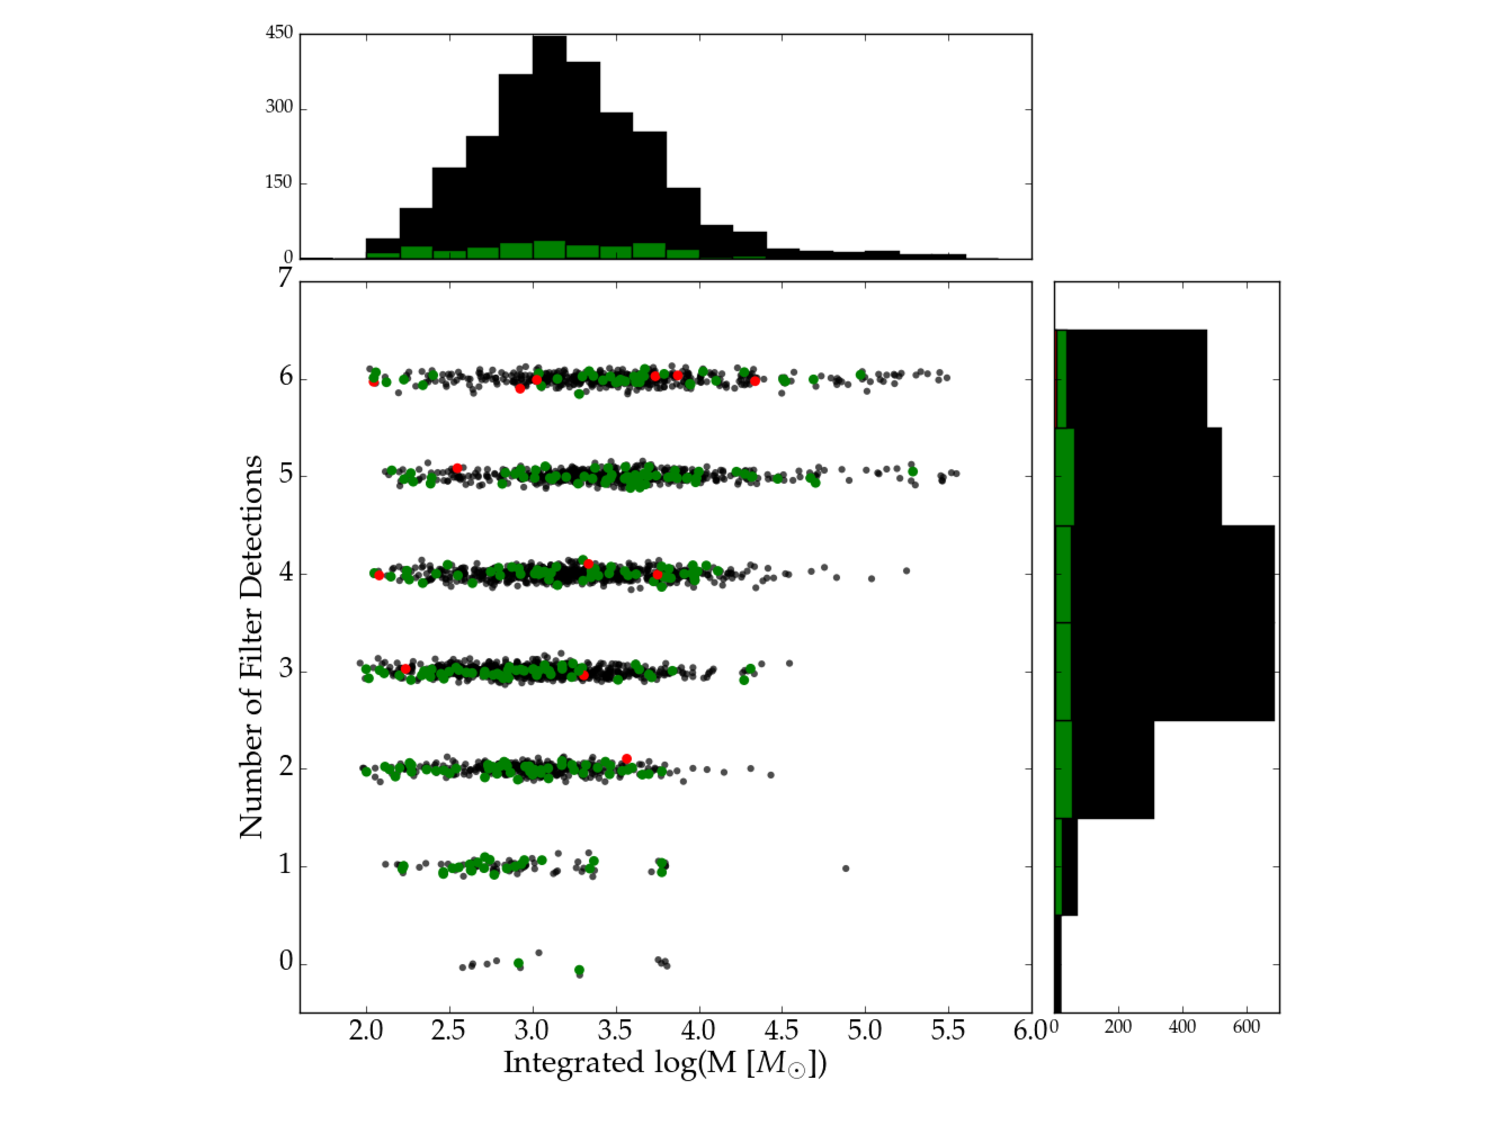
\includegraphics[trim=3.2cm 0.8cm 0.2cm 0.2cm, clip=True, scale=0.45]{plot_flag_ndet.pdf} 
      \end{array}$
   \end{center}
  \caption{Integrated $log_{10} (M)$ versus the number of filter detections where all flagged clusters are shown in red.  Histograms on sides show distributions of each.  A small amount of Gaussian scatter was added in the $y$-direction for clarity.}
  \label{fig:ndet}
\end{figure}



\section{Analysis of Results}
From here forward, we use the final adopted ages and masses in Table~\ref{table} to investigate properties of the cluster distributions.  We first characterize the broad properties of the cluster sample.  We then consider how these properties would change if only integrated measurements were available, as is the case for studies of more distant cluster populations.


\subsection{Age and Mass Distributions}\label{sec:distributions}


Now that we have ages and masses assigned to each cluster, we can look at the global distributions of these properties.  In Figure~\ref{fig:age_mass} we show the final results for age versus mass, color-coded by $A_{V}$.  There is a large range in both age and mass for our cluster sample, getting down to a few hundred solar masses, much lower than in other extragalactic cluster samples.  We see that there are no old, low mass clusters as expected from models of cluster dissolution \citep[e.g.,][] {Bastian06}, and even if they do exist, they would likely fall below our detection limit.  We also find no old highly reddened clusters, whereas young clusters have large range of extinction, which is consistent with them often being located in gas rich regions with active star formation.  Additionally, we do not observe any young massive clusters, which we should have detected if they actually exist.  This could indicate M31 was more efficient at forming massive clusters in the past.


\begin{figure}[!ht]
   \begin{center}$
      \begin{array}{cc}
         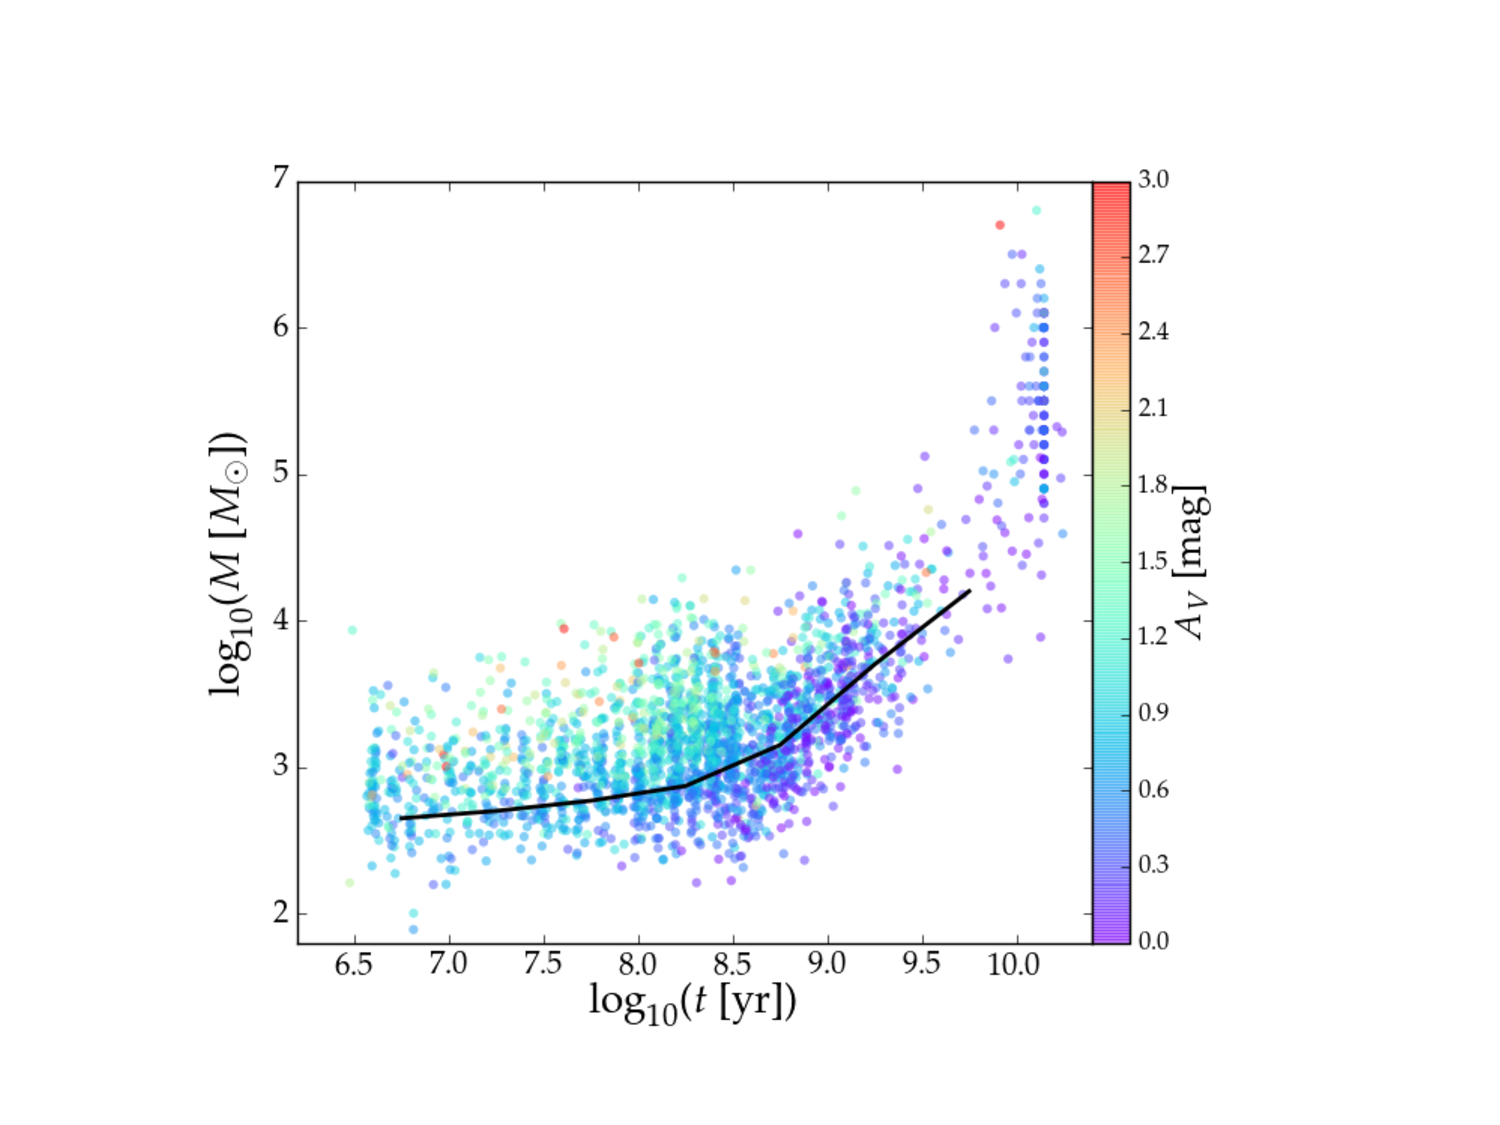
\includegraphics[trim=3cm 1cm 1cm 0.5cm, clip=True, scale=0.5]{age_mass_comp1018.pdf} 
      \end{array}$
   \end{center}
  \caption{Age versus mass for the final cluster results, color-coded by extinction.  Clusters labelled 'Not sure' are excluded.  The black line shows the 50\% completeness mass in for that age (from \citep{Johnson15}).}
  \label{fig:age_mass}
\end{figure}


\begin{figure}[ht!]
   \begin{center}$
      \begin{array}{cc}
         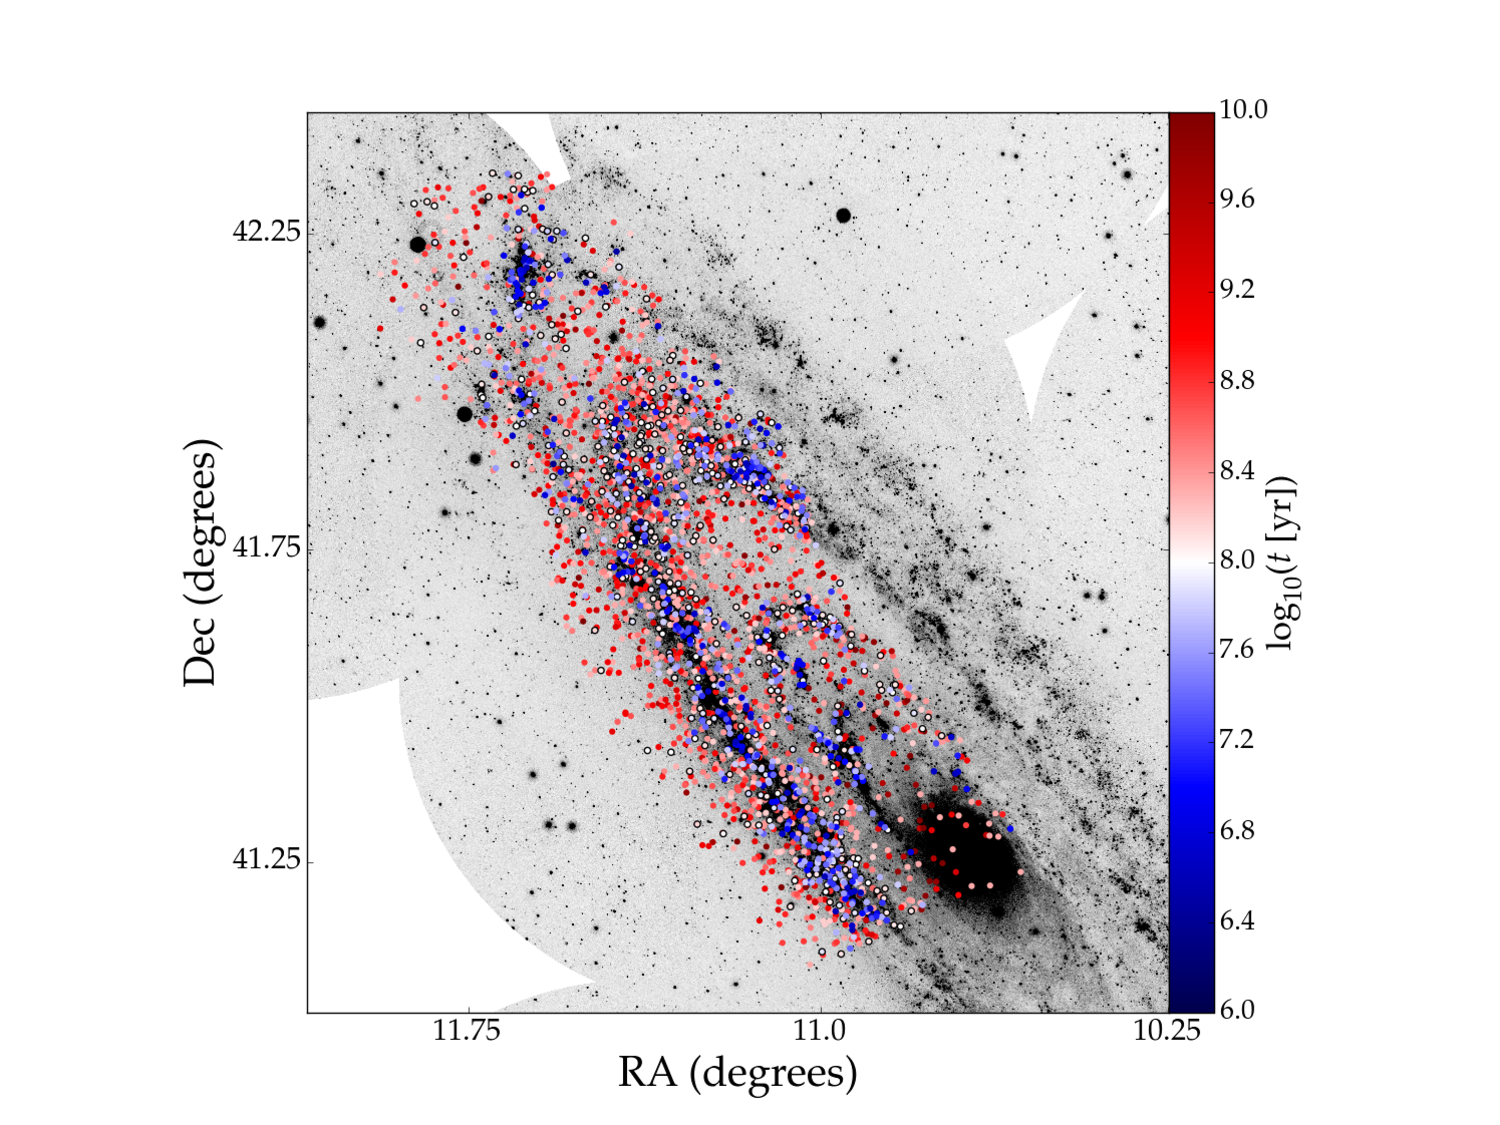
\includegraphics[trim=3.1cm 0.2cm 3cm 1.5cm, clip=True, scale=0.48]{cluster_catalog63.pdf} 
      \end{array}$
   \end{center}
  \caption{PHAT cluster locations shown on the GALEX NUV image \citep{Thilker05}, where the clusters are color-coded by age.  The youngest clusters (blue) lie mostly along the 10 kpc star-forming ring.}
  \label{fig:age_catalog}
\end{figure}


\begin{figure}[ht!]
   \begin{center}$
      \begin{array}{cc}
         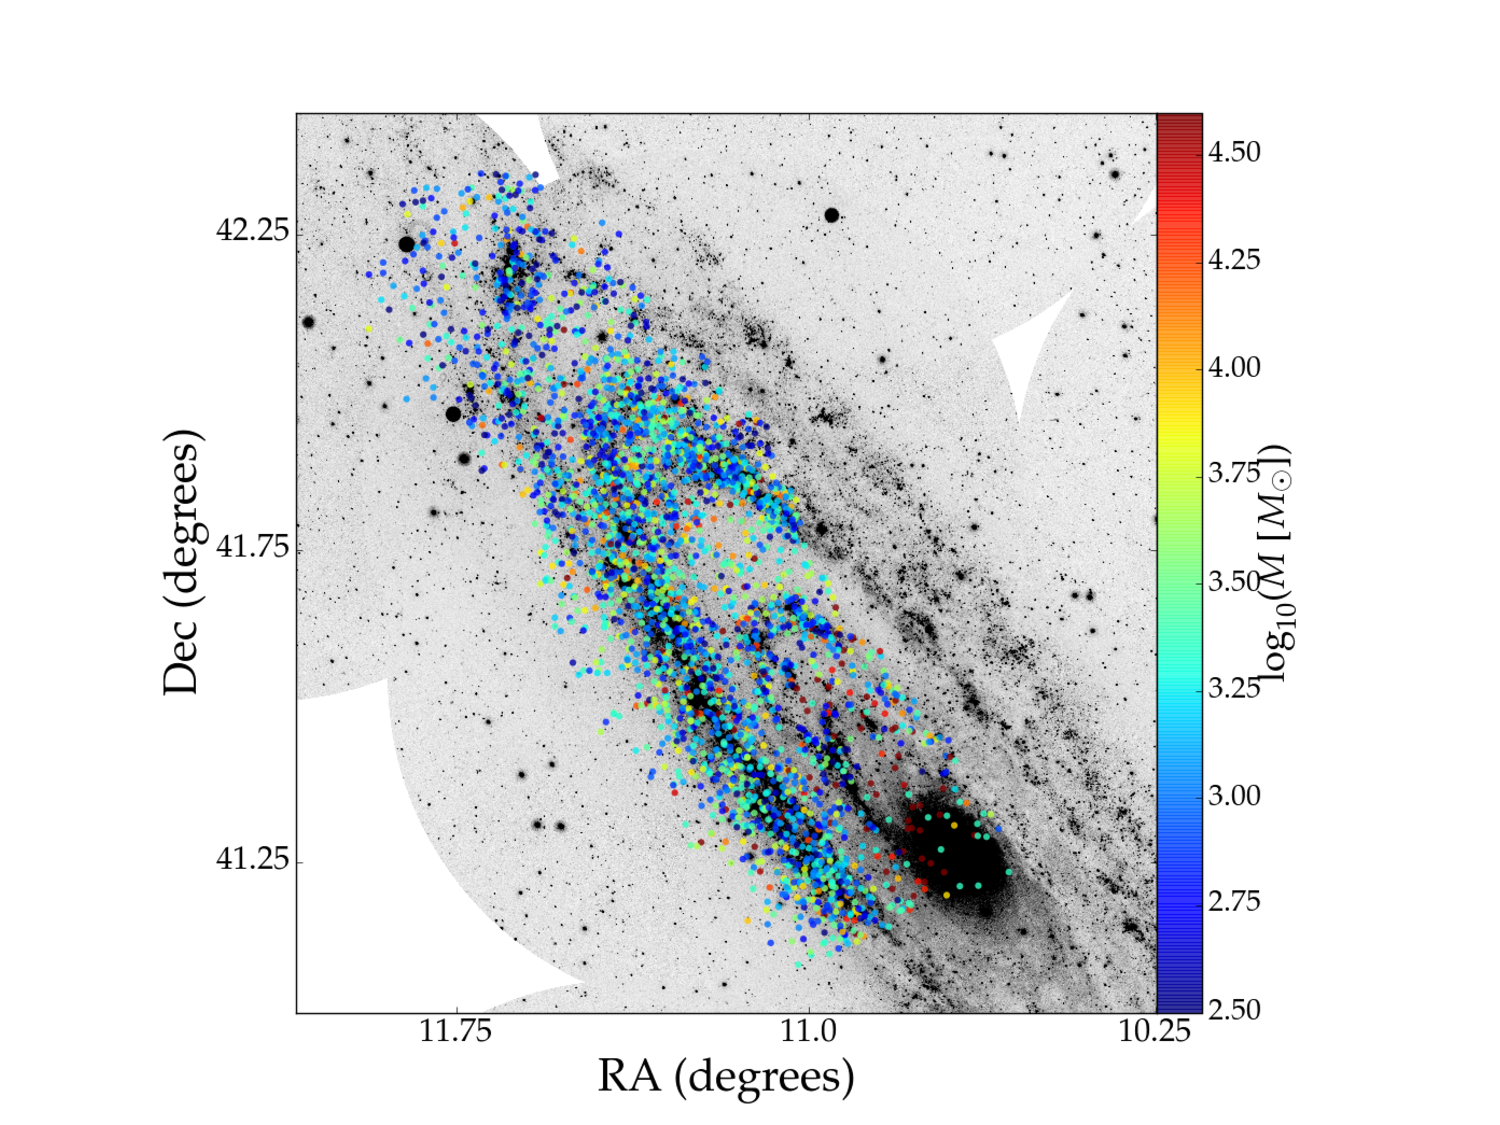
\includegraphics[trim=2.7cm 0.2cm 3cm 0.2cm, clip=True, scale=0.48]{cluster_catalog_mass63.pdf} 
      \end{array}$
   \end{center}
  \caption{PHAT cluster locations shown on the GALEX NUV image \citep{Thilker05}, where the clusters are color-coded by mass.  The massive clusters (red) lie mostly in the bulge, while lower mass clusters are spread throughout the disk.}
  \label{fig:mass_catalog}
\end{figure}


\begin{figure}[ht!]
   \begin{center}$
      \begin{array}{cc}
         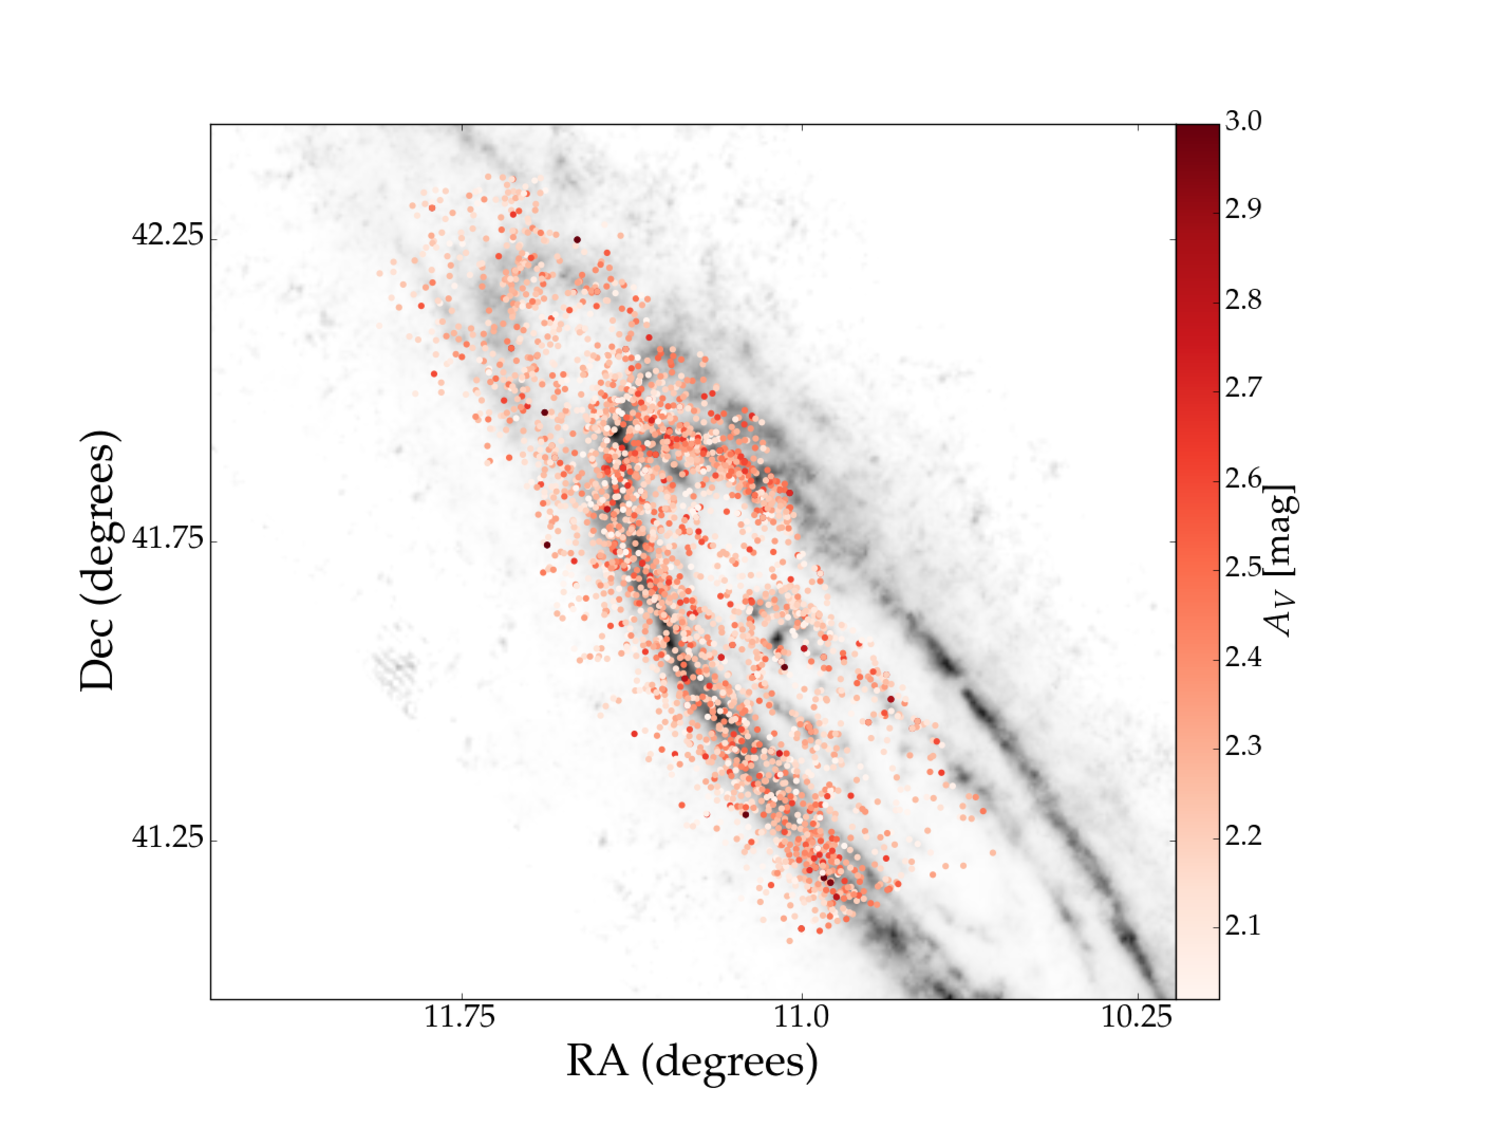
\includegraphics[trim=1.3cm 0.2cm 3cm 0.2cm, clip=True, scale=0.42]{cluster_catalog_av63.pdf} 
      \end{array}$
   \end{center}
  \caption{PHAT cluster locations shown on the dust map \citep{Draine07} image, where the clusters are color-coded by extinction.  The more reddened clusters (red) are mostly coincident with dusty regions.}
  \label{fig:av_catalog}
\end{figure}


In Figure~\ref{fig:age_catalog} we show the cluster locations on a background GALEX NUV image, where the clusters are color-coded by age.  The youngest clusters, shown in blue, trace the 10 kpc star-forming ring, while clusters found in the bulge region are older.  Figure~\ref{fig:mass_catalog} shows the cluster locations color-coded by mass, where more massive clusters are in red.  The massive clusters lie predominantly in the bulge, while lower mass clusters are spread throughout the disk.  Figure~\ref{fig:av_catalog} shows the cluster locations color-coded by extinction, over the M31 dust map.  The more reddened clusters, shown as darker red, are mostly coincident with dusty regions, as expected.



\begin{figure}[ht!]
   \begin{center}$
      \begin{array}{cc}
         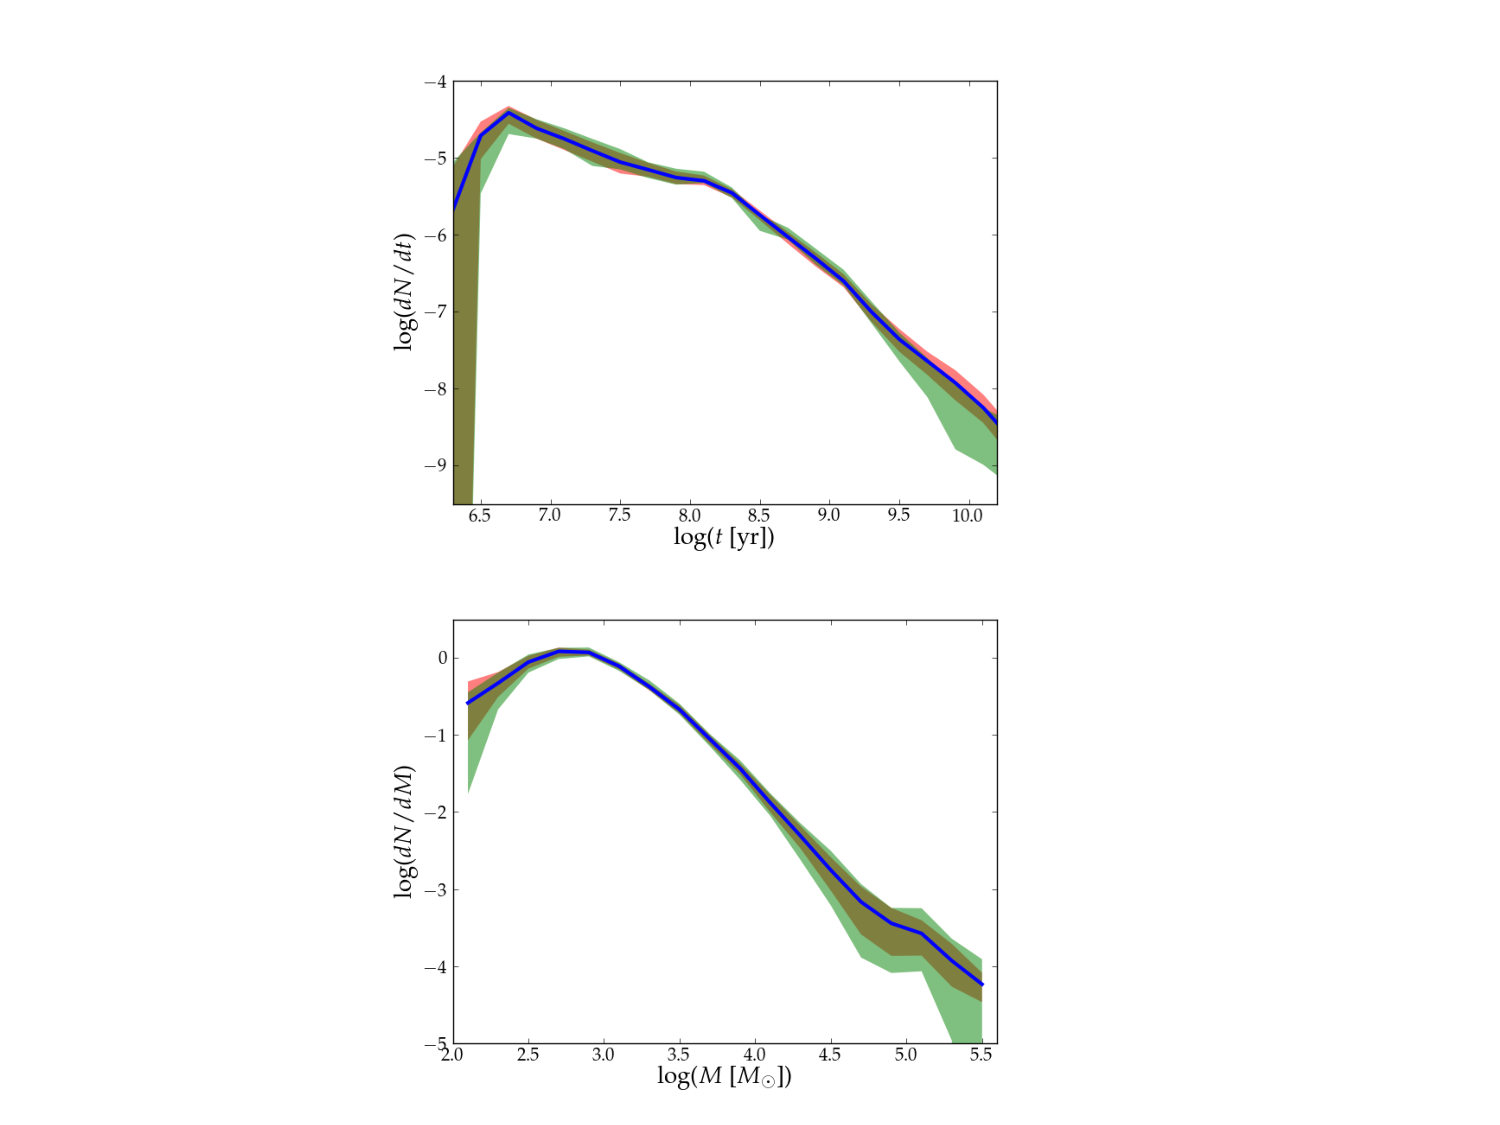
\includegraphics[trim=6.2cm 0.2cm 0.2cm 0.2cm, clip=True, scale=0.75]{all_dist.pdf} 
      \end{array}$
   \end{center}
  \caption{Present day age distribution (top panel) and mass distribution (bottom panel) as a function of cluster mass for the entire cluster sample.  Orange shaded regions represent uncertainties uncertainties that arise from uncertainties in the parameter fits, and the green shaded regions represent the uncertainties from the bootstrap resampling as described in the text.}
  \label{fig:distributions}
\end{figure}




In Figure~\ref{fig:distributions} we plot the present day age distribution (top panel - number of clusters per age bin, scaled by the width of each bin) and mass distribution (bottom panel - number of clusters per mass bin, scaled by the width of each bin).  Figure~\ref{fig:agedist} shows the age distribution for several slices in cluster mass, and Figure~\ref{fig:massdist} shows the mass distribution for several slices in cluster age.  These are marginal distributions, meaning that the age distribution is summed up over all masses and extinctions, and the mass distribution is summed up over all ages and extinctions.  

\begin{figure*}[!htbp]
   \begin{center}$
      \begin{array}{cc}
         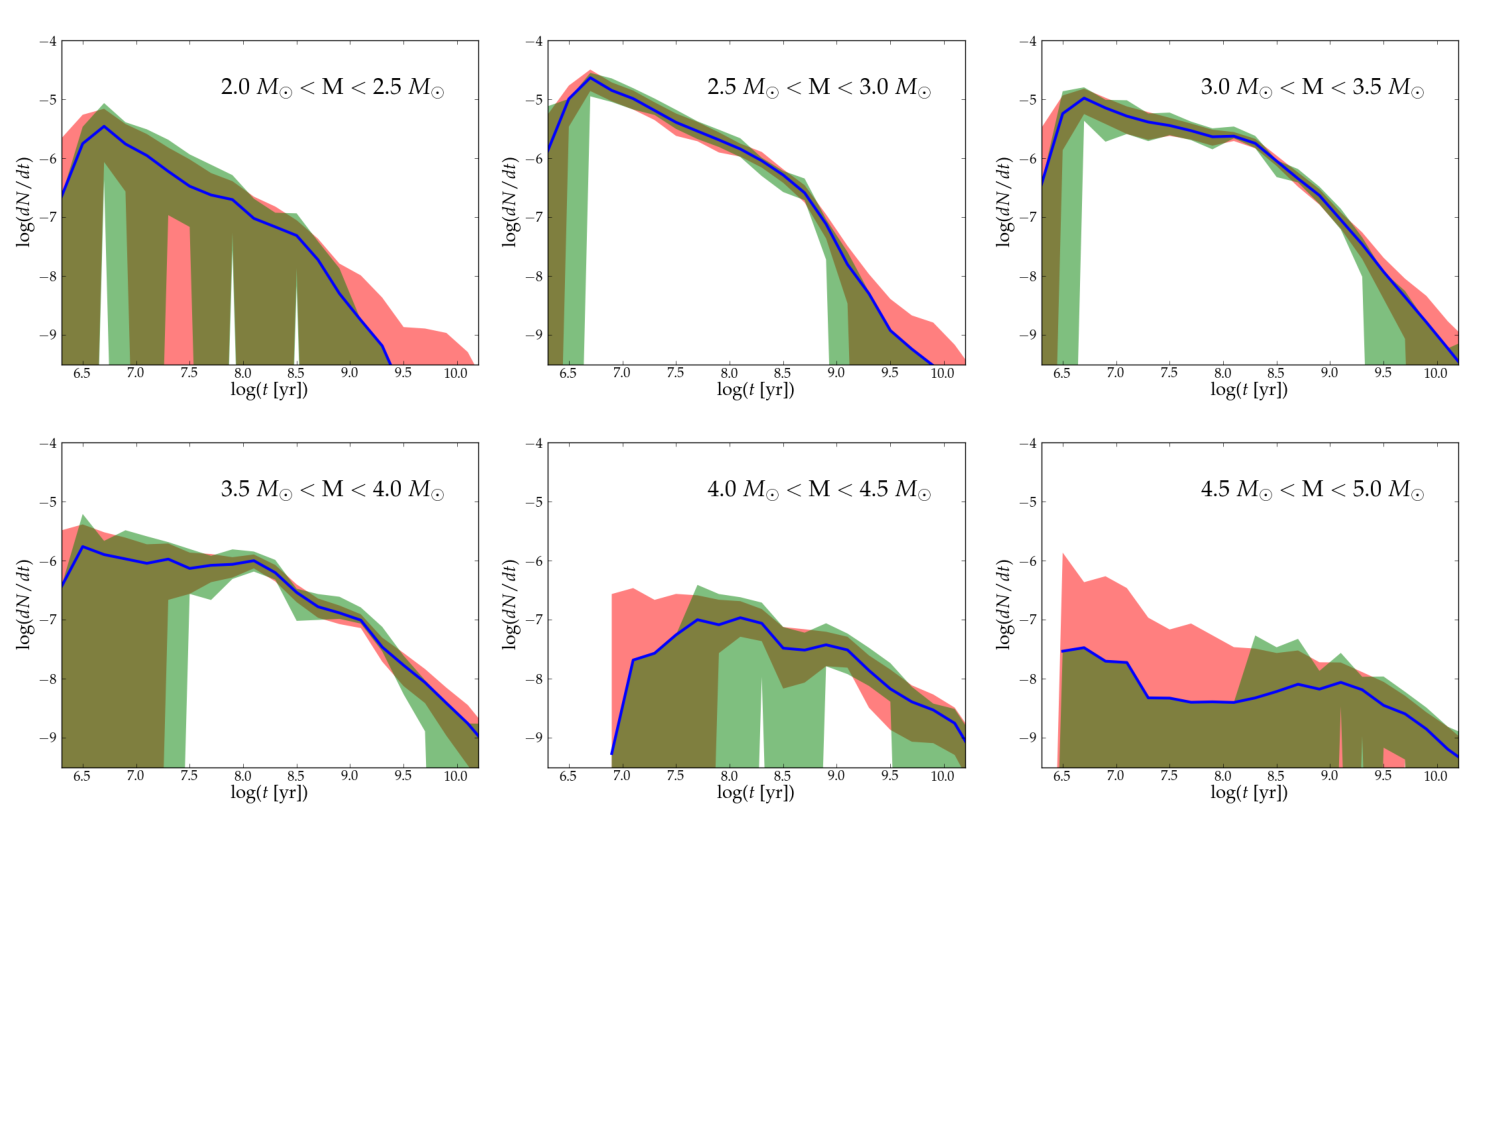
\includegraphics[trim=0.3cm 4.8cm 0.2cm 0.2cm, clip=True, scale=0.63]{age_dist_all.pdf} 
      \end{array}$
   \end{center}
  \caption{Present day age distribution as a function of cluster age for several slices in cluster mass.  Orange shaded regions represent uncertainties that arise from uncertainties in the parameter fits, and the green shaded regions represent the uncertainties from bootstrap resampling.}
  \label{fig:agedist}
\end{figure*}

There are two main sources of uncertainty when calculating these distributions:  uncertainty in the fitting procedure and uncertainty in the random sampling of clusters.  To account for the first, we make use of the information in the PDFs of each cluster.  Using only a best fit value would not yield an accurate global distribution since many clusters have wide or multiple peaked PDFs.  Additionally, summing the PDFs for each individual cluster assumes the PDFs are Gaussian, which is often not accurate.  Instead, we draw 1000 Monte Carlo samples from the PDF of each cluster.  We then calculate the mean and the standard deviation of the Monte Carlo draws for each cluster.  These means are binned in equal log spacing in age and mass to come up with the distributions shown, where the binned value for the means are represented by the blue lines, and the minimum and maximum values, representing the fitting uncertainties, are shown as the red regions.  These fitting uncertainties are shown as the red regions in the distribution plots and tend to be lower than the sampling uncertainties.  

\begin{figure*}[!htbp]
   \begin{center}$
      \begin{array}{cc}
         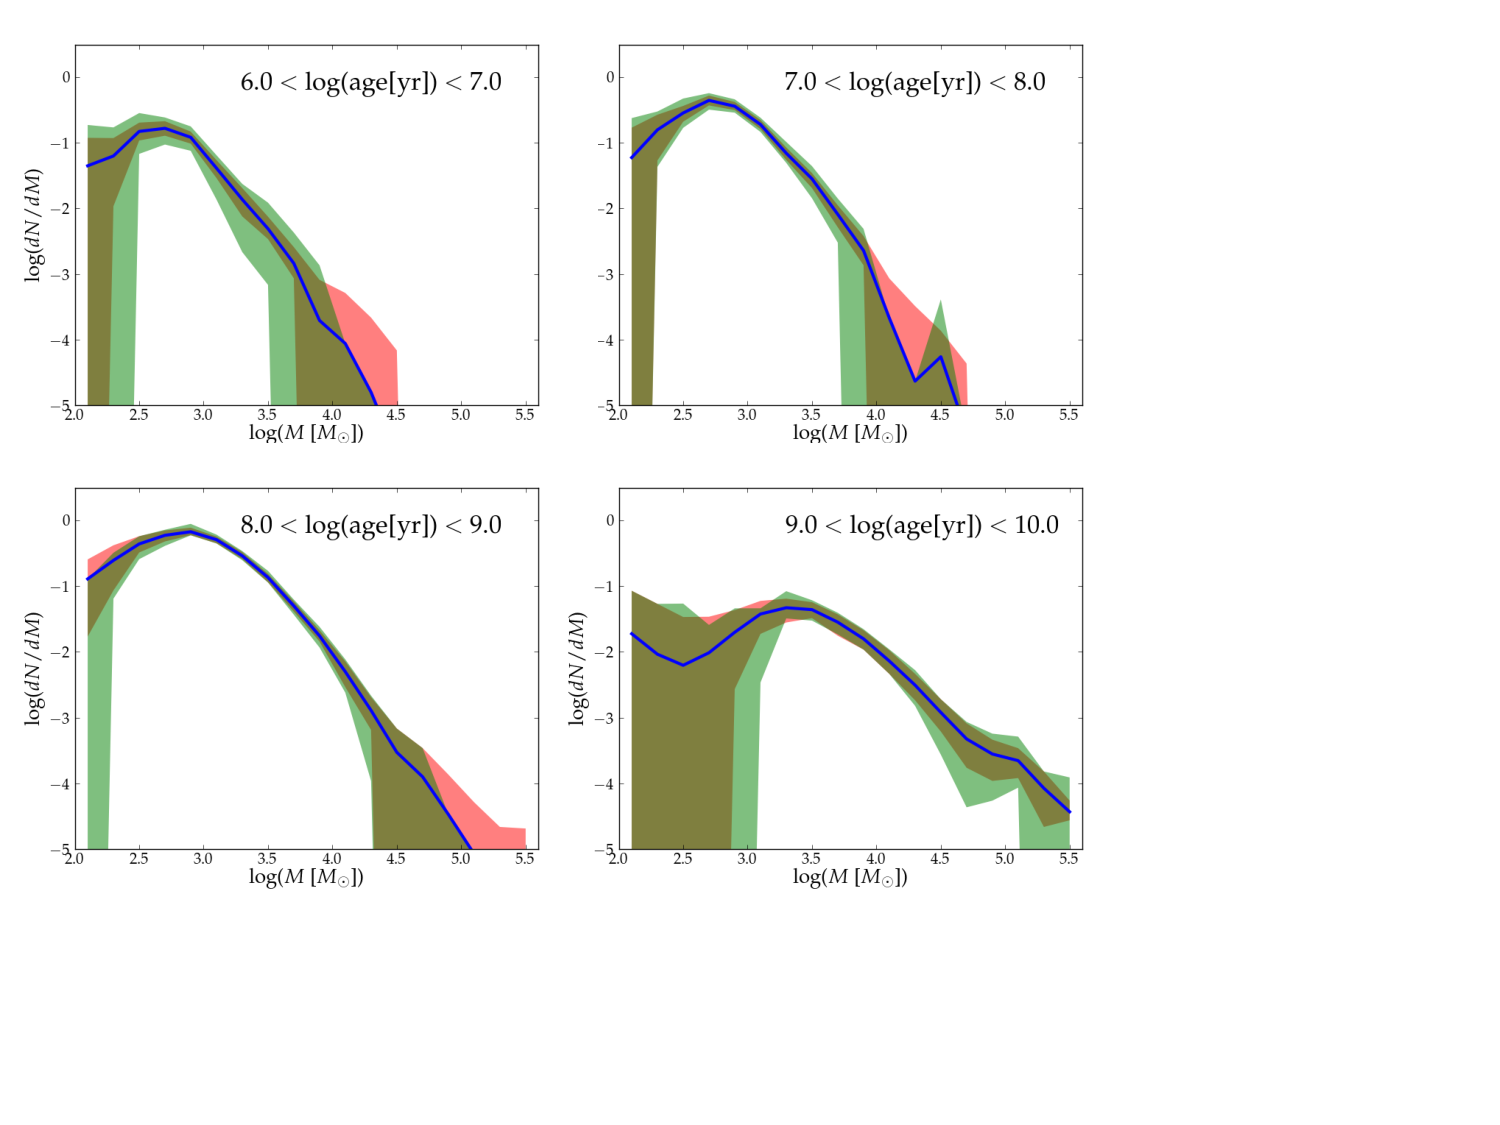
\includegraphics[trim=0.3cm 3cm 7cm 0.2cm, clip=True, scale=0.65]{mass_dist_all.pdf} 
      \end{array}$
   \end{center}
  \caption{Present day mass distribution as a function of cluster age for several slices in cluster age.  Orange shaded regions represent uncertainties uncertainties that arise from uncertainties in the parameter fits, and the green shaded regions represent the uncertainties from the bootstrap resampling as described in the text.}
  \label{fig:massdist}
\end{figure*}


To assess the sampling uncertainties due to the finite number of clusters, we perform bootstrap resampling, where we draw a random realization of the cluster sample 1000 times \citep[e.g.,][] {Fouesneau14}.  We derive the age and mass distributions for each of these realizations, and we take the minimum and maximum of these distributions as the sampling uncertainties, which are shown as the green shaded regions.  The sampling uncertainties are largest where there are fewer clusters, namely at older ages and at the high and low mass ends.  For the mass distribution, sampling uncertainty dominates  the parameter uncertainty for the whole distribution, since the mass determinations are fairly well constrained as compared to the age determinations.

For the the age distribution, we see that uncertainties in the parameter fits dominate at the youngest ages, while sampling uncertainties dominate at the oldest ages, where there are few clusters.  Sampling uncertainties also dominate at the poorly populated high mass end, while the two sources of uncertainty are similar in scale for the lower mass clusters.

The present day age distribution depends on several physical effects:  the cluster formation history, cluster dissolution, and selection effects.  The decline in the number of clusters at older ages is most likely a combination of these effects.  These distributions are largely power laws, and are broadly consistent with expectations and results of the smaller \cite{Fouesneau14} sample.  There is a roll over to low masses/ages consistent with sample incompleteness.  Distributions will be analyzed completely in Fouesneau et al (in prep).  Note that these are the complete observed distributions, and are not corrected for completeness, which also explains the large sampling uncertainties.   The sample is highly complete for M \textless\ $10^{3.2}M_{\odot}$ and $t$ \textgreater\ 10 Myr.  The turnover seen at lower masses and ages is in incomplete region, therefore the validity of this turnover is inconclusive.  A full analysis of cluster dissolution will be presented in Fouesneau (in prep).




\subsection{Using Integrated Cluster Photometry at Larger Distances}\label{sec:intonly}

Most extragalactic systems are too distant for us to resolve their individual stars, and thus only have integrated photometry available.  Now we revisit the results from the previous section and investigate how they would have changed had we only used integrated photometry.




\begin{figure}[ht!]
   \begin{center}$
      \begin{array}{cc}
         \includegraphics[trim=6.2cm 0.2cm 0.2cm 0.2cm, clip=True, scale=0.75]{int_dist.pdf} 
      \end{array}$
   \end{center}
  \caption{Present day age distribution (top panel) and mass distribution (bottom panel) as a function of cluster mass using only the results of the integrated light fitting.  Orange shaded regions represent uncertainties that arise from uncertainties in the parameter fits, and the green shaded regions represent the uncertainties from the bootstrap resampling as described in the text.  The black dashed lines show the median of the distributions using the most reliable parameters as plotted in Figure~\ref{fig:distributions}.}
  \label{fig:intdist}
\end{figure}


In Figure~\ref{fig:intdist} we show the overall marginalized age and mass distributions for the integrated fits only.  Figure~\ref{fig:intagedist} shows the integrated age distribution for several slices in cluster mass, and Figure~\ref{fig:intmassdist} shows the integrated mass distribution for several slices in cluster age.  The uncertainties were calculated as described in Section~\ref{sec:distributions}.

We can compare these figures directly with Figures~\ref{fig:distributions}, \ref{fig:agedist}, and \ref{fig:massdist} to see how the inferred distributions would change given only integrated fitting results.  The overall age distributions both show evidence for a turnover at the youngest ages, although this is in an incomplete region.  The integrated age distribution shows a dip around 20-30 Myr that the age distribution in Section~\ref{sec:distributions} does not show.  In Figure~\ref{fig:intagedist} we see that the dip in the age distribution between 10 and 100 Myr is primarily from clusters \textless\ $10^3 M_{\odot}$.  These young low mass clusters are strongly affected by stochasticity.  However, such clusters will be too faint to be detected in more distant samples.

The overall mass distributions are similar to each other in the region where we are complete (above $10^{3.2} M_{\odot}$), however the mass distribution in Section~\ref{sec:distributions} shows a turnover at the lowest masses, while the integrated mass distribution appears flat for the mass range below $\sim$ $10^{3.2} M_{\odot}$.  Figure~\ref{fig:intmassdist} shows that the mass distribution for the youngest clusters appears to turn over at low masses, similar to what is seen in the overall distribution for the fiducial distribution.  However for ages between 10 Myr and 1 Gyr the distributions appear to be flat at the lowest masses.  



\begin{figure*}[!htbp]
   \begin{center}$
      \begin{array}{cc}
         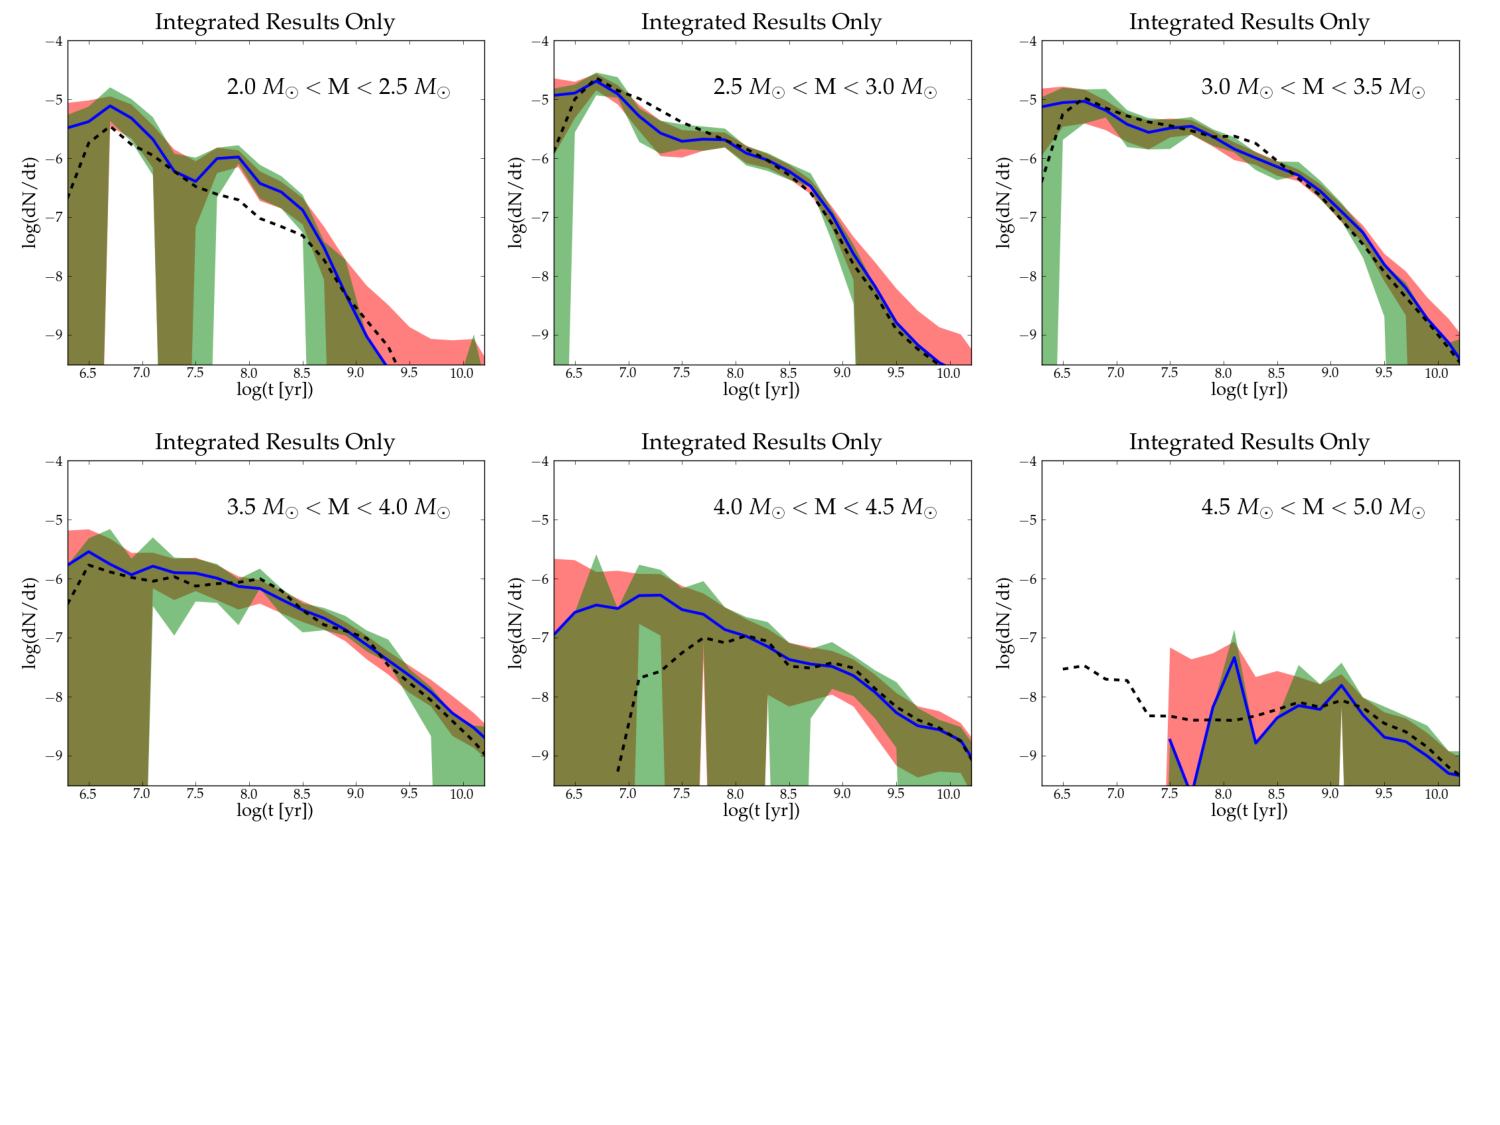
\includegraphics[trim=0.3cm 4.8cm 0.2cm 0.2cm, clip=True, scale=0.63]{age_dist_int.pdf} 
      \end{array}$
   \end{center}
  \caption{Present day age distribution as a function of cluster age for several slices in cluster mass using the results of the integrated light fitting.  Orange shaded regions represent uncertainties that arise from uncertainties in the parameter fits, and the green shaded regions represent the uncertainties from the bootstrap resampling as described in the text.  The black dashed lines show the median of the distributions using the most reliable parameters as plotted in Figure~\ref{fig:agedist}.}
  \label{fig:intagedist}
\end{figure*}



\begin{figure*}[!htbp]
   \begin{center}$
      \begin{array}{cc}
         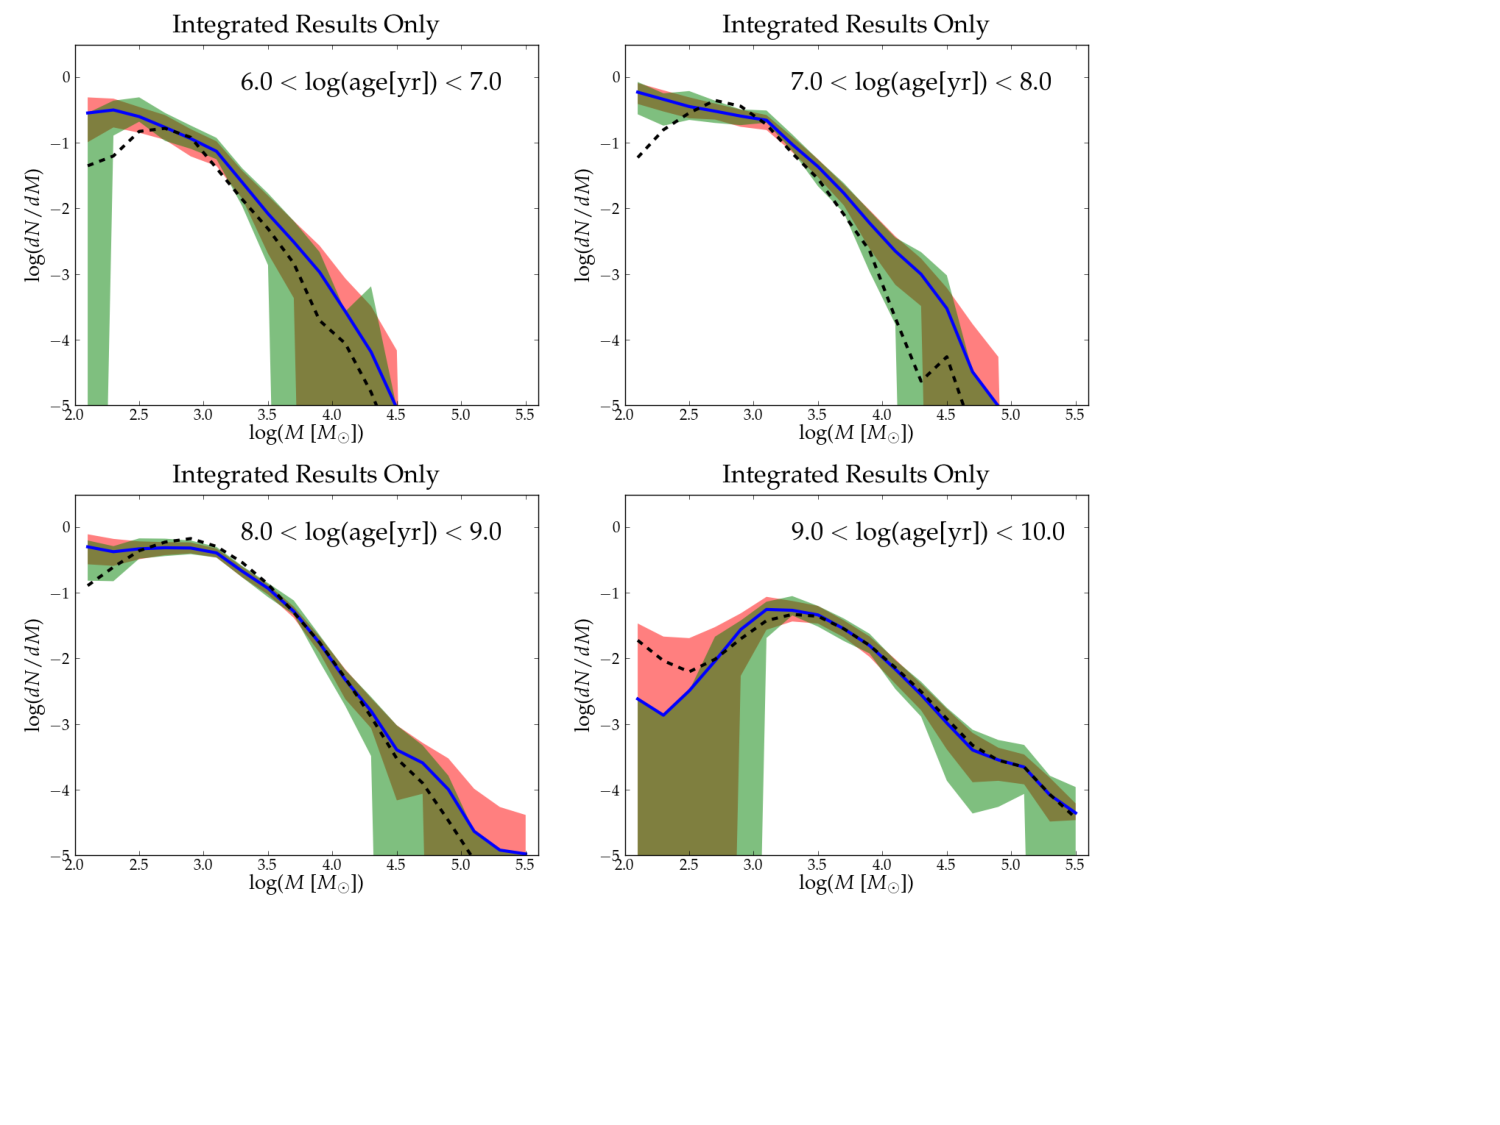
\includegraphics[trim=0.3cm 3cm 7cm 0.2cm, clip=True, scale=0.65]{mass_dist_int.pdf} 
      \end{array}$
   \end{center}
  \caption{Present day mass distribution as a function of cluster mass for several slices in cluster age using the results of the integrated light fitting.  Orange shaded regions represent uncertainties that arise from uncertainties in the parameter fits, and the green shaded regions represent the uncertainties from the bootstrap resampling as described in the text.  The black dashed lines show the median of the distributions using the most reliable parameters as plotted in Figure~\ref{fig:massdist}.}
  \label{fig:intmassdist}
\end{figure*}


In Figure~\ref{fig:intdiff} we show the difference in density between our fiducial results for the cluster sample and the integrated light results in each age-mass bin scaled by the square root of the number of clusters in each bin.  From this plot we can investigate which regions of parameter space change when we have only integrated light measurements.  At older ages, there is not much difference between the integrated results and the results from Section~\ref{sec:assign} since we used the integrated results for most clusters older than 300 Myr.  At younger ages, the integrated results under predicts the number of intermediate mass clusters at 100 Myr.  It also predicts fewer clusters of $\sim$ 1000 $M_{\odot}$ overall, and a slightly larger number of very low mass ($\sim$ 200 $M_{\odot}$) clusters. 


\begin{figure}[ht!]
   \begin{center}$
      \begin{array}{cc}
         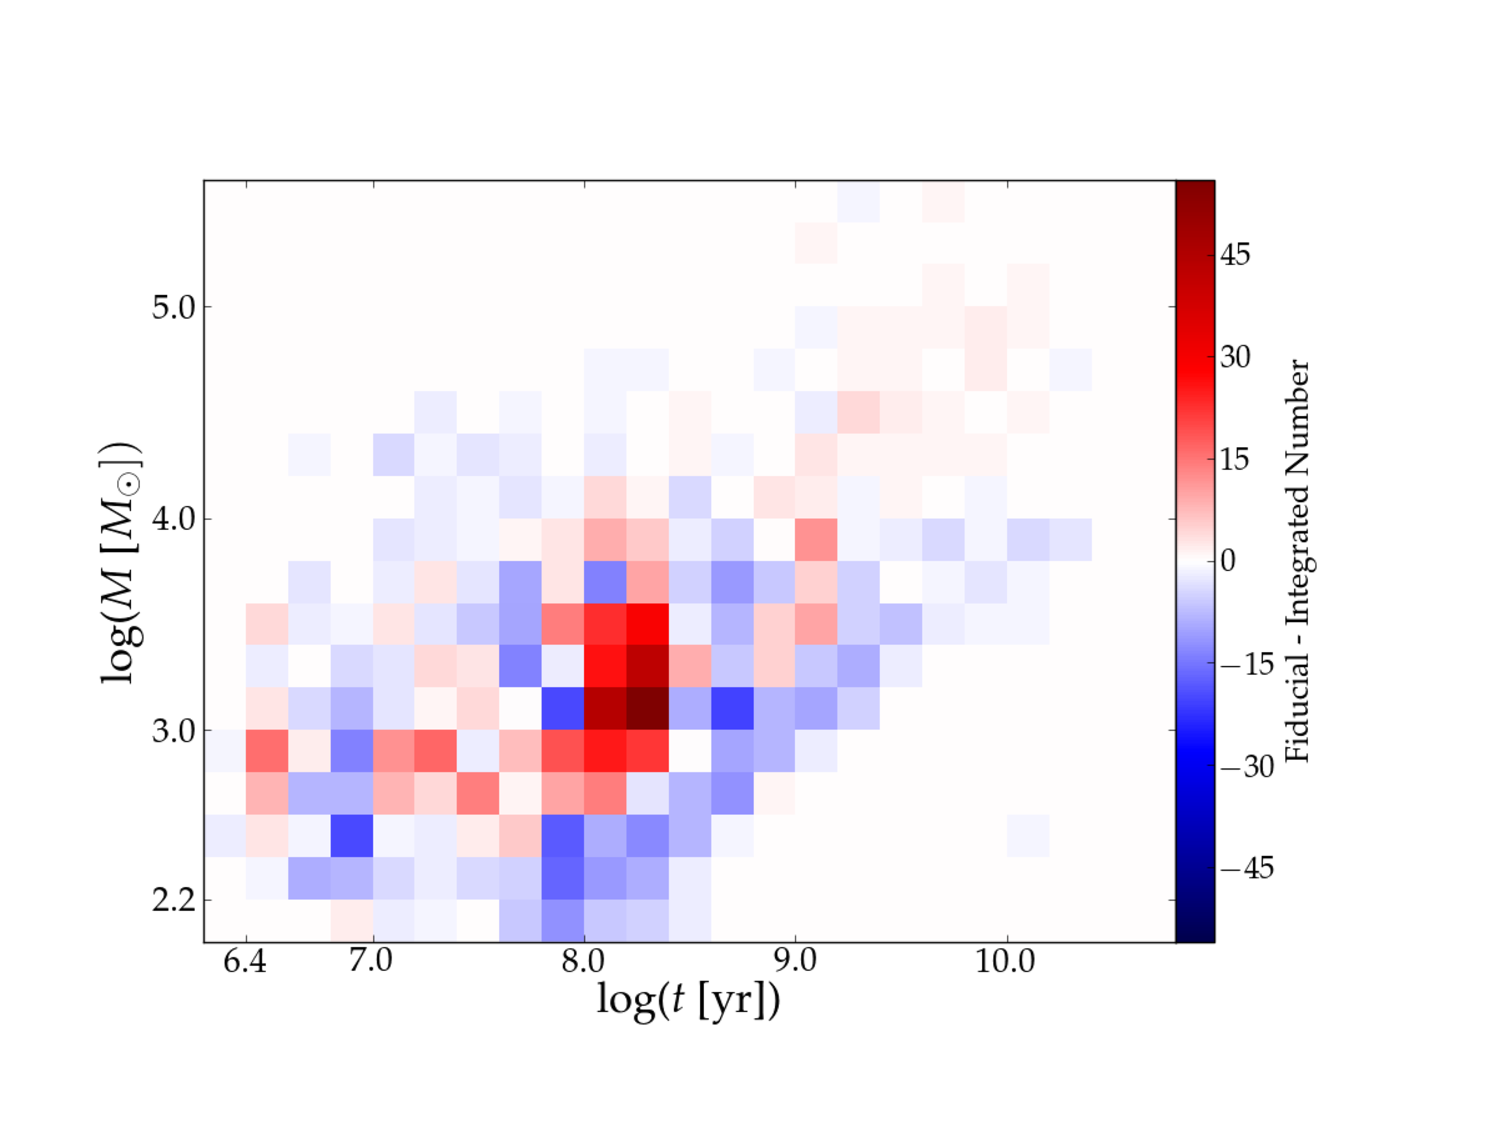
\includegraphics[trim=1.5cm 0cm 1cm 3cm, clip=True, scale=0.4]{int_diff62.pdf} 
      \end{array}$
   \end{center}
  \caption{Difference (optimal - integrated) in the number density between our fiducial results for the cluster sample and the integrated light results in the age-mass parameter space, where red is where there are more of the fiducial clusters in that bin and blue is where there are more integrated clusters in that bin.}
  \label{fig:intdiff}
\end{figure}

\section{Conclusions}\label{sec:conc}

We calculate ages, masses, and extinctions for 2753 clusters in the PHAT cluster sample using two methods:  CMD fitting and fitting integrated photometry to discrete models.  Tests on synthetic clusters show that the CMD fitting method recovers the parameters well for most clusters.  We did a by-eye check of which method is most accurate for each cluster and used this as our determination for the parameters.  Clusters in the sample range from a few hundred to $10^5 M_{\odot}$, 6 Myr - 10.2 Gyr, and 0 - 3 $A_V$.  This represents a large range in cluster properties, and allows us to use this sample for many studies of clusters that require completeness over a large mass range.

In general, we find that for clusters less than about 300 Myr, the CMD fitting method is most accurate.  For clusters older than this, many of their stars have evolved off the main sequence, and the turnoff falls below our detection limit, making it difficult to accurately fit models to the CMD.  In contrast, integrated models do a better job when clusters are older and stochastic effects are not as drastic.

We plot the present day age and mass distributions for the cluster sample, utilizing Monte Carlo techniques to account for uncertainties in the parameter determinations as well as the sampling.  These distributions show a lack of young massive clusters as well as old, low mass clusters.  Comparison to the integrated light only distributions shows that the general trends are recovered well, while there may be some differences in incomplete regions of parameter space.




%----------------------------------------------
\acknowledgements


{The authors wish to acknowledge the collective efforts of the entire PHAT team in this project.  This research made extensive use of NASA's Astrophysics Data System Bibliographic Services.  Support for this work was provided by NASA through grant number HST-GO-12055 from the Space Telescope Science Institute, which is operated by AURA, Inc., under NASA contract NAS5-26555.}

%Also, the authors thank the anonymous referee for a prompt and useful report.  

%----------------------------------------------

\bibliographystyle{apj}  \bibliography{Paper3_ref}

%--------------------------------------------------------------------



\end{document}

